%input macros (i.e. write your own macros file called MacroFile1.tex)
%\newcommand{\PdfPsText}[2]{
  \ifpdf
     #1
  \else
     #2
  \fi
}

\newcommand{\IncludeGraphicsH}[3]{
  \PdfPsText{\includegraphics[height=#2]{#1}}{\includegraphics[bb = #3, height=#2]{#1}}
}

\newcommand{\IncludeGraphicsW}[3]{
  \PdfPsText{\includegraphics[width=#2]{#1}}{\includegraphics[bb = #3, width=#2]{#1}}
}

\newcommand{\InsertFig}[3]{
  \begin{figure}[!htbp]
    \begin{center}
      \leavevmode
      #1
      \caption{#2}
      \label{#3}
    \end{center}
  \end{figure}
}


%%% Local Variables: 
%%% mode: latex
%%% TeX-master: "~/Documents/LaTeX/CUEDThesisPSnPDF/thesis"
%%% End: 


\documentclass[oneside,12pt]{Classes/CUEDthesisPSnPDF}

\title{ANALYSIS OF LARGE SOCIAL NETWORKS TO INVESTIGATE INTRIGUING PATTERNS}

\author{by \\ \vspace{2mm}AJITESH JAYANTH ( USN- 1MS12IS011 ) \\ AKSHAY RAO AK ( USN- 1MS12IS013 ) \\ ANKITH MOHAN ( USN- 1MS12IS014 ) \\ G AKASH ROHIT ( USN- 1MS12IS037 ) \vspace{2mm}  }
\collegeordept{DEPARTMENT OF INFORMATION SCIENCE AND ENGINEERING}
\university{M S RAMAIAH INSTITUTE OF TECHNOLOGY}
\renewcommand{\submittedtext}{A report submitted to \\M S RAMAIAH INSTITUTE OF TECHNOLOGY \\ Bengaluru  \vspace{0.1in} \\IS811 SENIOR PROJECT   \\as partial fulfilment of the requirement for \\  }
\degree{Bachelor of Engineering (B.E) in Information Science and Engineering}
\degreedate{May 2016}
\guide{under the guidance of \\ KRISHNARAJ P M}

\hbadness=10000
\hfuzz=50pt

%\usepackage[square,sort,comma,numbers]{natbib}
\usepackage{watermark}
\usepackage{multirow}
\usepackage{graphicx}
\usepackage[numbers]{natbib}
\usepackage{fancyhdr}
\pagestyle{fancy}
\fancyfoot{}
\renewcommand{\footrulewidth}{0.4pt}
\lfoot{Information Science Engineering, MSRIT, Bengaluru}
\rfoot{\thepage}
%\fancyfoot[R]{\thepage}
\begin{document}

\renewcommand\baselinestretch{1.2}
\baselineskip=18pt plus1pt

\maketitle

\setcounter{secnumdepth}{3}
\setcounter{tocdepth}{3}

\begin{romanpages}
\begin{center}
\thispagestyle{empty}
\bfseries
\large{Department of Information Science and Engineering \\
M S Ramaiah Institute of Technology \\
Bengaluru - 54} \\
{ \vspace*{2mm}{{
\includegraphics [scale =0.5]{logo}} \par}}
\LARGE{CERTIFICATE} \\
\end{center}
\vspace{0.1in}
\large{
This is to certify that Ajitesh Jayanth (USN- 1MS12IS011) , Akshay Rao A K (USN- 1MS12IS013), Ankith Mohan(USN- 1MS12IS014) and G Akash Rohit (USN- 1MS12IS037) who were working for their \textbf{IS811 SENIOR PROJECT} under my guidance, have completed the work as per my satisfaction with the topic \textbf{Analysis Of Large Social Networks To Investigate Intriguing Patterns}. To the best of my understanding the work to be submitted in dissertation does not contain any work, which has been previously carried out by others and submitted by the candidates for themselves for the award of any degree anywhere.
} \\
\vspace{0.2in}
\small{
\begin{flushleft}
\begin{tabular}{lllllllllrl}
(Guide) & & & & & & & & &(Head of the Department)\\
Krishnaraj P M & & & & & & & & &Dr. Vijay Kumar B P\\
Assistant Professor, Dept. of ISE   & & & & & & & & &Professor \& Head, Dept. of ISE
\end{tabular}
\end{flushleft}
\vspace{0.1in}
\begin{flushleft}
\begin{tabular}{llllllllll}
 & (Examiner 1) & & & & & & & (Examiner 2)  \\
Name &  & & & &\\ \\
Signature & & & & &
\end{tabular}
\end{flushleft}}
% ------------------------------------------------------------------------


\begin{center}
\thispagestyle{empty}
\bfseries
\large{Department of Information Science and Engineering \\
M S Ramaiah Institute of Technology \\
Bengaluru - 54} \\
{ \vspace*{2mm}{{
\includegraphics [scale =0.5]{logo}} \par}}
\LARGE{DECLARATION} \\
\end{center}
\vspace{0.5in}
\large{
We hereby declare that the entire work embodied in this \textbf{IS811 SENIOR PROJECT} report has been carried out by us at M S Ramaiah Institute of Technology under the supervision of Krishnaraj P M. This Project report has not been submitted in part or full for the award of any diploma or degree of this or any other University.} \\
\vspace{0.5in}
\begin{flushleft}
\small{ AJITESH JAYANTH ( USN- 1MS12IS011 ) \\ AKSHAY RAO AK ( USN- 1MS12IS013 ) \\ ANKITH MOHAN ( USN- 1MS12IS014 ) \\ G AKASH ROHIT ( USN- 1MS12IS037 ) }
\end{flushleft}

% ------------------------------------------------------------------------



% Thesis Acknowledgements ------------------------------------------------


%\begin{acknowledgementslong} %uncommenting this line, gives a different acknowledgements heading
\begin{acknowledgements}      %this creates the heading for the acknowledgments


%\begin{center}
We wish to express our sincere appreciation and gratitude to the Department of Information Science and Engineering for their extended long-term support and giving us the opportunity to analyse the interactions and structure within a social network. We would like to extend our hearty gratitude to our Principal, Dr.~N V R Naidu, our HOD Dr.~Vijay Kumar B P and especially to our guide, Krishnaraj P M for his vast reserve of patience, knowledge, constant feedback and guidance. This project would never have been completed without the unending encouragement and devotion of our family and friends.
%\end{center}


\end{acknowledgements}
%\end{acknowledgmentslong}

% ------------------------------------------------------------------------

%%% Local Variables: 
%%% mode: latex
%%% TeX-master: "../thesis"
%%% End: 

\normalsize{
%% Thesis Dedictation ---------------------------------------------------

 %this creates the heading for the dedication page

\begin{center}
\textbf{This work is licenced under \\ Creative Commons Attribution-Noncommercial 2.5 India Licence}\end{center}


You are free 
\begin{itemize}
 \item {to Share: to copy, distribute and transmit the work}
  \item{to Remix: to adapt the work}
\end{itemize}

\vspace{0.25in}


Under the following conditions:

\begin{itemize}
 \item { Attribution: You must attribute the work in the manner specified by the author or licensor (but not in any way that suggests that they endorse you or your use of the work)}
  \item{Noncommercial: You may not use this work for commercial purposes}
\end{itemize}
     
\vspace{0.25in}
With the understanding that:
\begin{itemize}
 \item {Waiver: Any of the above conditions can be waived if you get permission from the copyright holder}
  \item{Other Rights: In no way are any of the following rights affected by the license}
  \subitem * {Your fair dealing or fair use rights;}
  \subitem * {The author's moral rights;}
  \subitem * {Rights other persons may have either in the work itself or in how the work is used, such as publicity or privacy rights.}
\end{itemize}

Notice: For any reuse or distribution, you must make clear to others the license terms of this work. 

\begin{flushleft}
(The complete legal code of the license is given in Appendix \ref{license} ) 
\end{flushleft}



% ----------------------------------------------------------------------

%%% Local Variables: 
%%% mode: latex
%%% TeX-master: "../thesis"
%%% End: 


% Thesis Abstract -----------------------------------------------------


%\begin{abstractslong}    %uncommenting this line, gives a different abstract heading
\begin{abstracts}        %this creates the heading for the abstract page

This project focuses on analysis of data related to social interaction among individuals in Free
and Open Source Software ecosystem. Undoubtedly this has emerged as a socially
important big data problem in recent times. The analysis discussed here includes four main topics,
namely, Weight Assignment, Influence Analysis, Link Prediction and Time Series Analysis.
Weight Assignment involves enhancement of the network structure in order to obtain
a real world perspective. On the other hand, Influence Analysis identifies the highly influential
individuals among the entities in a social network. Link Prediction deals with predicting
the most probable interactions in the future among individuals using already existing
interactions. Since social networks are not stationary objects, Time Series Analysis
is a dynamic approach used to formally understand the growth of
a network over time. These concepts are illustrated with analysis of certain large
social networks. Since the emphasis currently is on big data, a new technique based
on random sampling of subnetworks from very large networks is developed and tested.
All the computations and algorithms have been implemented on R and have been tested on a number of 
large datasets. Improvements in performance have been observed compared to existing methods. 
\end{abstracts}
%\end{abstractlongs}


% ----------------------------------------------------------------------


%%% Local Variables: 
%%% mode: latex
%%% TeX-master: "../thesis"
%%% End: 

\printnomenclature  
\tableofcontents
\listoffigures
\listoftables
}
\end{romanpages}
                                      
%%% Thesis Introduction --------------------------------------------------
\chapter{Introduction}
\ifpdf
    \graphicspath{{Introduction/IntroductionFigs/PNG/}{Introduction/IntroductionFigs/PDF/}{Introduction/IntroductionFigs/}}
\else
    \graphicspath{{Introduction/IntroductionFigs/EPS/}{Introduction/IntroductionFigs/}}
\fi

%\section{Motivation}
%\section{Scope}
%\section{Objectives}

\section{Motivation}
The rapid computerization and availability of high computing power have led to the emergence of social-networks.
A brief insight about the topological and behavioural aspects of complex networks can be achieved by a thorough
understanding of social networks. It is considered a very important topic for research due to the widespread
success of social networking websites such as Facebook, Twitter and Linked-in.

Social networks are structures where nodes represent people or entities and edges represent interaction,
influence or collaboration between entities. They grow and change quickly over time through the addition of
new edges, signifying the appearance of new interactions in the underlying social structure. Social network
analysis involves identifying mechanisms by which they grow and evolve. The major application of social
networks are point to point overlay networks, security systems in ad-hoc networks, hybrid sensor networks,
prediction and control of an epidemic, cellular telephone systems and it also helps us to predict links
in the world wide web or any other given computer network.

\section{Objectives}
Social network analysis is our primary focus wherein we follow practices such as design, analysis, coding,
testing and maintenance so that the evolution of the network can be observed over time. Huge data-sets are
collected and assimilated which signify interaction between two or more social entities thus providing insights
regarding how closely related they are, at what instance of time they interact and the duration of the
interaction. The underlying concept or the phenomenon has to be proved by various methodologies such as
algorithmic analysis either in a iterative or in a regressive fashion followed by modelling, visual representation,
animation and detailed presentation.

Obtaining of preliminary results sheds some light on the very fact whether this approach gives us comprehensive
and satisfying results in the near future. The underlying concept is proof-tested by applying on various data-sets
obtained from heterogeneous sources. The results and findings from this experimental set-up help to identify
relationships among social entities, derive patterns and accurately predict the future outcomes. Detailed
results are obtained, thus enabling us to conclude their significance in a real world environment.

The interest of this project lies in social networking concepts such as social influence analysis,
time series analysis, link prediction, cluster analysis, small world phenomenon and power law analysis.

\section{Elements of Network Analysis}

\subsection{Social Network Analysis (SNA)}

Increase in the use of personal computers in late 1980s has encouraged much wider use of SNA  methods because it has meant increased ability to manage large data sets and to visualize social network data in a wide variety of ways. Social network analysis (SNA) is the analysis of social networks. A social network is a social structure made up of a set of social actors (such as individuals or organizations) and a set of the dyadic ties between these actors.

The social network perspective provides a set of methods for analysing the structure of whole social entities as well as a variety of theories explaining the patterns observed in these structures. The study of these structures uses social network analysis to identify local and global patterns, locate influential entities, and examine network dynamics.

Social Network Analysis is the study of social relations among a set of actors. It concerns the network structure formulation and solution. Such structures are usually captured in graphs. Limelight on analysis was thrown very recently; until then it was invisible even to the organizations which depend on them. Every organisation has a network within itself since network is nothing but relationships among interacting units.

Social network analysis has now emerged from being a suggestive metaphor to an analytic approach to a paradigm, with its own theoretical statements. It has gained a significant following in anthropology, biology, communication studies, economics, geography, information science, organizational studies, social psychology and many other fields. In organisations collaboration in networks is critical to innovation. Paradoxically these networks are taken for granted, frequently invisible and rarely managed.

Social network analysis is focused on uncovering the patterns of people’s interactions. A rapid growth in work across organisation as well as geographic boundaries with outsourcing, off-shoring, virtual organisations and business process networks, combined with trends such as the rise of blogs, online communities and social networking sites such as Friendster and LinkedIn as well as the rapid growth of collaborative software have all contributed to the emergence of Social Network Analysis (SNA) from the academic closet.

Social relationships are viewed in terms of network theory (consisting of nodes and connections) by social network analysis. These networks are often depicted in a social network diagram, where nodes are the points and ties are the lines. Social network analysis is based on an assumption of the importance of relationships among interacting units.

The network’s perspective encompasses theories, models, and applications that are expressed in terms of relational concepts or processes. Along with growing interest and increased use of network analysis has come a consensus about the central principles underlying the network perspective.

Social Network Analysis (SNA) can be defined as a set of techniques underpinned by statistical analysis that make visible the hidden connections that are important for sharing information, decision-making and innovation in an organization.

\subsection{Concepts used by SNA}

Social network is the mapping and measuring of relationships and flows between people, groups, organizations, animals, computers or any other Information/Knowledge processing entities. Graphs, Matrices, Statistical Models and a few Formal methods like Graphical and Mathematical Models are used to visualize Social Networks. Maximum flow, Hubbell and Katz cohesion, Centrality and Power are the most influencing properties of a Social Network. Cliques, N-Clans and L-Plexes are the different Ideas used to study the Sub-Structures and Groups of a Social Network. The Web can be treated as a Social Network, weblogs as special subsets of web can also be considered as Social Networks. Page Rank in Google and HITS are a few Social Network Analyses applied on web contents for efficient search results for the user queries. The semantic web is an emerging concept that launches the idea of having data on the web defined and linked in a way that it can be used by people and processed by machines. The semantic web and social network models support each other.

\noindent {\bf Graph Mining}

Graphs have become extremely important in modelling complicated structures. Many domains produce data that can be intuitively represented by graphs. The process of discovering interesting facts and information about these graphs is difficult and challenging to work with because real world data is very huge for any sort of raw interpretation, so that graph mining which is a data mining approach has to be incorporated with SNA to obtain the results of the data sets so as to provide us with an insight of the frequent sub graphs of interest.

\pagebreak
\noindent {\bf Link Analysis}

Link mining works with graph structures that have nodes with defined set of properties. With more and more information becoming available today in databases, structured documents, plain texts, transcribed conversations, and sometimes even in non-verbal form, such as images and videos, the possibilities for link analysis, as well as the associated challenges, are growing by leaps and bounds. Link Prediction is a kind of Link Analysis technique used in SNA to find out the future links that are most likely to occur based on the analysis of the data.

\noindent {\bf Centrality and Betweenness}

Importance of each node in a Social Network is varied based on its influence in the whole network. Measuring the rank of a node in any large network is thus a very crucial task. Social Network Analysis helps to determine rank or the centrality of the actors according to their position in the social structure using the knowledge of connectivity. Betweenness Centrality (BC) helps to get a more precise rank of the actors in the network by involving more global information such as its role played in the existence of paths between any two given nodes in the network. Three heuristic algorithms are proposed for influential nodes selection after detecting communities in Social Networks. These algorithms outperform the greedy algorithm and traditional heuristics in terms of speed .

\noindent {\bf Density}

The density of a graph is the number of existing edges over the number of possible edges. It represents the connectedness of nodes in a graph. Higher density in graphs shows the most active regions and implies that more activities are occurring at exponential rates like new actors joining and new relations being formed. This leads to repeated analysis for new insights that can be obtained.


\noindent {\bf Clustering}

Clustering is the most important topic that deals with unsupervised data. It deals with finding a structure in a collection of unlabelled data. A cluster is therefore a collection of objects which are similar between them and are dissimilar to the objects belonging to other clusters. Hence, the goal of clustering is to determine the intrinsic grouping in a set of unlabelled data.

\pagebreak
\noindent {\bf Classification}

Classification is the supervised way of using known properties to categorize the data with unknown properties. In inter graph classification the graphs are classified under different labels based on the properties of the data inside graphs. Classification model is built using machine learning techniques based on the known properties of graphs, and the graphs with unknown properties are classified based on the model.

\noindent {\bf Average Path Length} 

In a network, the distance between two nodes is the number of edges in the shortest path connecting them. The diameter D is the maximal distance between any pairs of nodes. The average path length L is defined as the mean distance between any two nodes. It was an interesting discovery that the average path length of most real complex network is relatively small, even in those kinds of networks which have fewer edges than a globally coupled network with an equal number of nodes. This kind of smallness is inferred as small world effect. 

\noindent {\bf Clustering Coefficient} 

The common phenomenon of existence of the mutual friend concept is simply that two friends usually have a common acquaintance, or it so happens that a person gets to know another person through a friend. This property naturally leads to clustering inside a given network where we come across the concept of clustering coefficient C. This can be defined as the average fraction of pairs of neighbours of a node that are also neighbours of each other. 

\noindent {\bf Degree Distribution} 

The most important feature of any given node is its degree. The degree is characterized by the total number of connections. Hence greater the degree of the network higher is the importance of that node in the network. The degree sequences obeys the Poisson distribution. The power law distribution falls off more gradually than an exponential one, allowing for a few nodes of very large degree to exist. As power laws are free of any characteristics scale, such a network with a power law degree distribution is called a scale free network. In order to analyse the small world phenomenon we make use of mathematical models and graphs. In one of the graphs we concluded that the logarithmic increase in average path length with the size of the network is typically a small world effect. This logarithmic graph gives us a better essence and understanding of complex networks. A very important concept, `richer become richer' is exhibited in complex network systems where all nodes concentrate at a given point.

\noindent {\bf Applications of SNA}

\begin{itemize}
\item Civil society organizations use SNA to uncover conflicts of interest in hidden connections between government bodies, lobbies and businesses, Network operators (telephone, cable, mobile) use SNA-like methods to optimize the structure and capacity of their networks
\item Businesses use SNA to analyse and improve communication flow in their organization, or with their networks of partners and customers
\item Law enforcement agencies (and the army) use SNA to identify criminal and terrorist networks from traces of communication that they collect; and then identify key players in these networks
\item Computer scientists have used network analysis methods to study webpages, Internet traffic, information dissemination, etc.
\item Social Network Sites like Facebook use basic elements of SNA to identify and recommend potential friends based on friends-of-friends
\item Social Network Analysis is used to determine influential journalists and analysts in the IT industry.
\item Mapping executive’s personal network based on email flows can be done using Social Network Analysis.
\end{itemize}


\noindent {\bf Small World Phenomenon}

An experiment conducted by a social psychologist Stanley Milgram during 1960 in the United States of America in order to find the average path lengths of social networks made use of small world type of networks. The aim of the experiment was to study the complexity of communication when a given message was exchanged between any two random people living in different parts of the country, that is
when a source person had to deliver a message to a target person. Milgram himself with a set of other mathematicians, handed out letters to people in Boston, and these people were asked to deliver the given letter to a target person in Massachusetts whose personal information such as name occupation and address was given but the letters had to be passed on as fast as possible to another person whom they knew but on only a first-name basis. 

After the experiment concluded it was found that at most five or six people were involved in the exchanging of most of the messages (short chains of acquaintances), hence the phrase six degrees of separation, here at least two of them being intermediaries. It was concluded that the given letter would reach faster if the given person was socially accessible and affluent. It was also inferred that there existed very short paths between arbitrary nodes. Individuals having local information are very suited for finding these paths. Milgram’s work was considered to be the first empirical evidence of social networks. The most critical fact of this experiment is that such short paths can be also seen in social networks which helps us to successfully analyse a huge set of given data.

It is still considered a very important topic for research due to the widespread of social networking websites such as Facebook, MSN messenger or due to the importance of social networks in general. Advent of many natural and complex networks has stimulated a great deal of interest in the concept of small world and the principles underlying them. Networks are structures of nodes or vertices connected by links or edges, for example, the World Wide Web. Rapid computerization of data and availability of high computer power have led to the emergence of complex networks and social networks in general.

In small-world we come across exponential networks or homogeneous networks in which the network size peaks at an average value and then goes on to decay exponentially, it is so because of the same number of link connections. An observation was made in the field of complex networks in which large scale complex networks are scale free which means their connectivity distributions are in a power law form, which means they are independent of the network scale. The main difference between a scale free network and exponential network is that most nodes have very few link connections and yet a few nodes have many connections. With the help of scale free networks and small world it gives us a brief insight about the topological and behavioural aspects of complex network.  

The major application of the small world phenomenon are point to point overlay networks, security systems in ad hoc networks, hybrid sensor networks, prediction and control of an epidemic, cellular telephone systems and it helps us to predict links in the world wide web or any given computer network.

\noindent {\bf Power Law}

A Power Law is a mathematical relationship between two quantities, where one quantity varies as a fixed power of another. A network whose degree distribution follows a power law is called a scale-free network. A graph for power law follows a long/heavy tailed distribution. The power law graph can be used to demonstrate the ranking of popularity of nodes and predict the region of interest of a particular node in a network. The procedure for verifying power law for a network is a dynamic approach, where data are analysed over a period of time.

\noindent {\bf Link Prediction}

Given a snapshot of a social network, can we infer which new interactions among its members are likely to occur in the near future? This question is formalized as the link prediction problem, and we develop approaches to link prediction based on measures for analysing the proximity of nodes in a network. Experiments on large co-authorship networks suggest that information about future interactions can be extracted from network topology alone, and that fairly subtle measures for detecting node proximity can outperform more direct measures.

The task of predicting links that are either missing or may appear in the future is addressed by link prediction. The methods proposed to cope with the link prediction problem are divided into two categories: unsupervised and supervised methods. Unsupervised methods assign a score for each pair of nodes using either local or global neighbourhood information. Experimental results on different social networks show that these methods are time consuming and are not feasible for large social networks. Supervised methods on the other hand consider link prediction as a classification problem. It uses different network information such as structural properties of the network, node attributes to determine the link existence between a pair of nodes. However, it does not use other information such as behaviour of nodes. It concentrates only on the existence of the links and not the properties of individuals that the nodes represent. In order to overcome such drawbacks, hybrid methods are developed which consider local information as well as community information.

Given a network, the probabilities of link existence and nonexistence of all the links in the network are computed. To determine the probability of a non-existent link, a hybrid method is established which uses Bayesian theory. For the weighted relationships among the nodes in a large network, the probabilities of existence of any link in the network are computed. Next, clustering is performed to obtain the different communities present in the network. For pairs of nodes which are not linked, the number of common neighbours between the nodes within and outside of their communities are determined.

From the parameters calculated so far, the posterior probabilities of link existence and nonexistence for the pairs of nodes are computed. A similarity score for the pairs of nodes is calculated as the ratio of posterior probability of link existence to the posterior probability of nonexistence. The computed scores are sorted in decreasing order to show that links with higher probability will come into existence earlier than those with lower probabilities.

\noindent {\bf Clustering}

One of the most important applications of graphs is to represent real systems as a graphical network so as to detect community structure, or clustering, i.e. the organization of vertices in clusters, with many edges joining vertices of the same cluster and comparatively few edges joining vertices of different clusters. Such clusters, or communities, can be considered as fairly independent compartments of a graph. Being able to identify these sub-structures within a network can provide insights into how network function and topology affect each other. Such insights can be useful in improving some algorithms on graphs such as spectral clustering. Various clustering methods exist based on statistical
and machine learning techniques. Some of the most useful methods are discussed and applied in later
sections.

Detecting communities is of great importance in sociology, biology and computer science, disciplines where systems are often represented as graphs.


\noindent {\bf Weight Assignment}

It is necessary to obtain a clear perspective of the networks to carry out effective analysis. In general, networks can be weighted or un-weighted. The drawback of using un-weighted networks is the lack of real world representation. Therefore the analysis of these networks is difficult. Hence it is necessary to assign weights to the ties among the nodes in a network. Weights are assigned to the edges by considering the features of the network and properties of graph theory. The network features include timestamps, influence, interactions, relationships and emotions. The properties are centrality, betweenness, clustering coefficient and power-law behaviour. In some cases it is useful to come up with alternative definitions of centrality, cohesiveness and affinity. 


\noindent {\bf Influence Analysis}

An attempt is made using social network analysis to answer the question, ”Who are the most influential individuals in a network?” Influential individuals are said to be those who are capable of convincing other individuals to adapt their attitude, behaviour, or belief to that of the former. Identifying the key influential individuals in a network can play a key role in the introduction, longevity, and fidelity of program implementation.


\noindent {\bf Time Series Analysis}

Time series analysis is an approach for data analysis where the data is assumed to arrive
sequentially over time. This is indeed the correct approach if the process which is generating the
data is evolving over time, rather than staying static. Special techniques are needed here
since the model used are different.

%%% ----------------------------------------------------------------------


%%% Local Variables: 
%%% mode: latex
%%% TeX-master: "../thesis"
%%% End: 

%\section{Literature Review}
\subsection{Analysis of Complex Weighted Social Networks}

In this section the role of edge-weights in a social network is briefly surveyed. The drawback of using plain networks (without weights) is, it does not provide meaning in the real world sense. Therefore the analysis of these types of networks becomes very difficult. Hence it is necessary to assign weights to the ties between the nodes in a network. The weights are assigned to the edges by considering the features of the network and also identifying alternative definitions for the properties of graph theory. The benefits of this improvisation are:-
\begin{itemize}
\item Helps to find better methods for analysis
\item Obtain accurate results after analysis
\item Helps in better visualisation
\end{itemize}

The outcome of this process helps in predicting links and finding influential nodes in an efficient way.

Numerous networked structures can be found in different contexts such as technology, transportation infrastructure, social phnomenon and biological systems. These networks are very complex in nature and are heterogeneous in their capacity and intensity among connections. Before, These features were not considered for studies because links were represented either as present or absent. The two main example networks suitable for study are Scientific Collaboration network(SCN) and World-Wide Air transportation Network(WAN). These networks can be better analysed by assigning weights to the edges proportional to the intensity and capacity of the connections among the nodes. Appropriate metrics are defined to characterize the complex statistical properties and topological observations. The results provides a better insight into the structural heirarchies and descriptions.
The weights are assigned to the edges by considering both the properties of graph theory and the features of the network. The properties are centrality, betweenness, clustering coefficient and power-law behaviour. In some cases it is useful to come up with alternative definitions of centrality, cohesiveness and affinity. The conclusions show a more complete view of the complex networks. The importance of correlation between weights and topology of the networks is appreciated because it provides a better perpective of the network and these details cannot be obtained by the quantities just based on topological information. The study thus offers a quantitative and general approach to understand the complex architecture of real weighted networks.\cite{Barrat2004}

Feature weighting is an important application in content-based recommender systems. In content-based recommender systems, the main attributes are assigned weights. These weights are assigned based on their importance to users. A set of linear regression equations are used to estimate the weight values. These equations are obtained from social network graphs and are judged based on similarity of items.
In content based recommendation system, every item is represented as an attribute or a feature. These features hold numerical or nominal values. The similarity of two items is computed using various distance measures between features. The similarity values are then used to obtain a ranked list of recommended items. The edges are assigned different weights based on human judgement. A formula for computing similarity can be derived by using weights and function of attributes. The feature weights are estimated from social network graphs. A network is constructed using the results of existing recommender with items as nodes. The similarity among items can be induced using optimal feature weights. These optimal feature weights can be determined from linear regression equations. Thus feature weighting provides effective results from the recommender systems leading to rigorous analysis.\cite{Debnath2008}

{\bf Role of edge weights} 

The structure of social networks influence the various dynamic processes of human interactions and communication. Weighted network models help to emulate the structure of real social networks They also help in displaying community structures with weak and strong internal links connecting the communities. The edge weights not only are important for dynamic processes but also in the formation of network structure itself. Weighted social networks can be designed to yield proper weight-topology correlations. They help to generate opinion formation models. Link weights not only make the model more realistic for describing human interactions in a social network but also generate a clear community structure. Thus it can be concluded that interaction weights play an important role in social dynamics. \cite{Toivonen2007}

{\bf Method : Attribute weight assignment}

This component mainly aims to assign a weight to each attribute in a network. It allows to represent attribute importance within a defined context. The assignment of weights depends on the framework created for the network structure. It can be assigned manually or computed automatically. Manual assignment allows users to include their preferences and inputs. Automatic assignment is provide to allow considering the social network characteristics. However, both can be used. The weight assignment to attributes is based on Inverse Functional Property(IFP). An algorithm can be designed for the process of assigning weights to attributes. The important steps of the algorithm are:

\begin{itemize}
\item Computing the importance of each attribute by crawling the related social networks.
\item Convert the input data into useful representation.
\item Computing the similarity score between each pair of similar attributes.
\item Data analysis step
\item Associating each attribute with a set of similarity scores inorder to compute the final weight.
\end{itemize}

Data aggregation/fusion techniques are needed to combine information from different sources and obtain one result for a more accurate decision. These techniques several approaches such as probabilistic models, evidence theories and classical functions. An important application of attribute weight assignment is profile matching in social networks.  It also helps in better understanding of inter-social network operations and functionalities. \cite{Raad2010}

{\bf Example:}
A scientific collaboration network is considered for analysis. The strength of collaborative ties are estimated. A formula for assigning weights to the edges is devised by making suitable assumptions. Social network analysis algorithms are applied on the weighted network and the results are examined. The improvements in the performance of SNA algorithms on weighted networks are observed and reasons for the same are stated. \cite{Newman2001}

@book{ross2014introduction,
  title={Introduction to probability models},
  author={Ross, Sheldon M},
  year={2014},
  publisher={Academic press}
}

%% Chapter1 has Literature Review
\chapter{Literature Review}
\ifpdf
    \graphicspath{{Chapter1/Chapter1Figs/PNG/}{Chapter1/Chapter1Figs/PDF/}{Chapter1/Chapter1Figs/}}
\else
    \graphicspath{{Chapter1/Chapter1Figs/EPS/}{Chapter1/Chapter1Figs/}}
\fi


\section{Analysis of Complex Weighted Social Networks}

In this section the role of edge-weights in a social network is briefly surveyed. The drawback of using plain networks (without weights) is, it does not provide meaning in the real world sense. Therefore the analysis of these types of networks becomes very difficult. Hence it is necessary to assign weights to the ties between the nodes in a network. The weights are assigned to the edges by considering the features of the network and also identifying alternative definitions for the properties of graph theory. The benefits of this improvisation are:-
\begin{itemize}
\item Helps to find better methods for analysis
\item Obtain accurate results after analysis
\item Helps in better visualisation
\end{itemize}

The outcome of this process helps in predicting links and finding influential nodes in an efficient way.

Numerous networked structures can be found in different contexts such as technology, transportation infrastructure, social phenomenon and biological systems. These networks are very complex in nature and are heterogeneous in their capacity and intensity among connections. Before, These features were not considered for studies because links were represented either as present or absent. The two main example networks suitable for study are Scientific Collaboration network(SCN) and World-Wide Air transportation Network(WAN). These networks can be better analysed by assigning weights to the edges proportional to the intensity and capacity of the connections among the nodes. Appropriate metrics are defined to characterize the complex statistical properties and topological observations. The results provides a better insight into the structural hierarchies and descriptions.
The weights are assigned to the edges by considering both the properties of graph theory and the features of the network. The properties are centrality, betweenness, clustering coefficient and power-law behaviour. In some cases it is useful to come up with alternative definitions of centrality, cohesiveness and affinity. The conclusions show a more complete view of the complex networks. The importance of correlation between weights and topology of the networks is appreciated because it provides a better perspective of the network and these details cannot be obtained by the quantities just based on topological information. The study thus offers a quantitative and general approach to understand the complex architecture of real weighted networks.\cite{barrat2004architecture}

Feature weighting is an important application in content-based recommender systems. In content-based recommender systems, the main attributes are assigned weights. These weights are assigned based on their importance to users. A set of linear regression equations are used to estimate the weight values. These equations are obtained from social network graphs and are judged based on similarity of items.
In content based recommendation system, every item is represented as an attribute or a feature. These features hold numerical or nominal values. The similarity of two items is computed using various distance measures between features. The similarity values are then used to obtain a ranked list of recommended items. The edges are assigned different weights based on human judgement. A formula for computing similarity can be derived by using weights and function of attributes. The feature weights are estimated from social network graphs. A network is constructed using the results of existing recommender with items as nodes. The similarity among items can be induced using optimal feature weights. These optimal feature weights can be determined from linear regression equations. Thus feature weighting provides effective results from the recommender systems leading to rigorous analysis.\cite{debnath2008feature}

\noindent {\bf Role of edge weights} 

The structure of social networks influence the various dynamic processes of human interactions and communication. Weighted network models help to emulate the structure of real social networks They also help in displaying community structures with weak and strong internal links connecting the communities. The edge weights not only are important for dynamic processes but also in the formation of network structure itself. Weighted social networks can be designed to yield proper weight-topology correlations. They help to generate opinion formation models. Link weights not only make the model more realistic for describing human interactions in a social network but also generate a clear community structure. Thus it can be concluded that interaction weights play an important role in social dynamics. \cite{toivonen2007role}

\noindent {\bf Method : Attribute weight assignment}

This component mainly aims to assign a weight to each attribute in a network. It allows to represent attribute importance within a defined context. The assignment of weights depends on the framework created for the network structure. It can be assigned manually or computed automatically. Manual assignment allows users to include their preferences and inputs. Automatic assignment is provide to allow considering the social network characteristics. However, both can be used. The weight assignment to attributes is based on Inverse Functional Property(IFP). An algorithm can be designed for the process of assigning weights to attributes. The important steps of the algorithm are:

\begin{itemize}
\item Computing the importance of each attribute by crawling the related social networks.
\item Convert the input data into useful representation.
\item Computing the similarity score between each pair of similar attributes.
\item Data analysis step
\item Associating each attribute with a set of similarity scores in order to compute the final weight.
\end{itemize}

Data aggregation/fusion techniques are needed to combine information from different sources and obtain one result for a more accurate decision. These techniques several approaches such as probabilistic models, evidence theories and classical functions. An important application of attribute weight assignment is profile matching in social networks.  It also helps in better understanding of inter-social network operations and functionalities. \cite{raad2010user}

\noindent {\bf Example:}
A scientific collaboration network is considered for analysis. The strength of collaborative ties are estimated. A formula for assigning weights to the edges is devised by making suitable assumptions. Social network analysis algorithms are applied on the weighted network and the results are examined. The improvements in the performance of SNA algorithms on weighted networks are observed and reasons for the same are stated. \cite{clauset2009power}

\section{Influence Analysis}\label{SecIA}

An attempt is made using social network analysis to answer the question ''Who are the most influential individuals in a network?''. Influential individuals are said to be those who are capable of convincing other individuals to adapt their attitude, behaviour, or belief to that of the former. Identifying the key influential individuals in a network can play a key role in the introduction, longevity, and fidelity of program implementation.
 
Given a set of weighted, directed relations among the individuals in a large network, clustering  based on the fast greedy algorithm \cite{clauset2004finding} is initially performed on this network to identify closely related sub-networks of individuals. Next, these clusters are analysed one by one as independent organizations. The PageRank \cite{brin1998anatomy} of all the individuals in the cluster are computed in order to determine their local standing (relative to  the cluster). For each individual A, the weights that A has assigned to every other individual in the cluster is multiplied by the PageRank of A in order to incorporate the influence of A. With these updated weights, the in-degree centrality (also known as in-ties) is computed and then used as a measure of the total communication directed at each individual. For each individual, the in-tie measure indicates how well other individuals in the cluster weigh this individual. Individuals who receive higher scores are considered more influential in the network.

In order to visualize the distribution of the in-degree measure within an organization, the in-degree scores for all individuals can be sorted in descending order and then graphed, resulting in a ''scree'' plot. This technique allows a researcher to get a sense of the distribution of in-ties for all the actors in the organization. Now the focus is on establishing a defensible threshold for identifying the most influential individuals in an organization. Visual inspection of the scree plot can make identifying influential’s an onerous task. As an alternative, four reproducible methods are investigated for categorizing influential individuals in an organization. A detailed explanation of these methods follows. These explanations and further details can be found in \cite{cole2009identifying}.

\noindent {\bf Method 1 - Absolute Cut Score}

The simplest and most intuitive method for determining a cut score is to set a predetermined absolute value above which individuals are deemed influential and below which they are not. Graphically, this can be accomplished by superimposing a horizontal line over the in-degree scree plot. Those individuals whose influence scores are above the horizontal line are then categorized as influentials. However, since this method is based entirely on a single point and is determined independent of variation in the distribution of in-ties, it can result in the situation where every individual (or no individual) in a network can potentially be deemed influential since the criterion is absolute, not relative.

\noindent {\bf Method 2 - Fixed Percentage of Population}

An alternative method of identifying influentials is to select a fixed percentage of the population as influential. If the top 20\% of individuals in an organization are to be categorized as influentials, this is equivalent to selecting the leftmost 20\% of the individuals in the graph. Those individuals to the left of a vertical line superimposed over the scree plot are categorised as influential. As with the Absolute Cut Score, this method identifies individuals as influential independent of the variation of in-ties. It ensures that a given percentage of individuals in the organization are identified as influential and their identification is based upon their performance relative to the performance of other individuals in the organization.

\noindent {\bf Method 3 - Standard Deviation}

Unlike the first two approaches, the Standard Deviation method focuses on the variation in the distribution of ties. This procedure requires calculation of the mean and standard deviation of the number of in-ties. Then we create a horizontal line two standard deviations above the mean, which can be superimposed over the scree plot. This horizontal line approach is similar to the Absolute Cut Score (Method 1), however, the Standard Deviation method does not choose a cut score a priori, instead it utilizes the observed data in determining where to set the cut point. Under this method, those individuals whose in-degree scores are above this line are marked ''influential.''

\noindent {\bf Method 4 - Random Permutation}

Through the use of random permutations, Method 4 produces results which identify those individuals who received significantly more in-ties than would have occurred by chance alone. This method capitalizes on the creation of a sampling distribution of potential networks that could have occurred, conditional on the fixed row marginal’s or (out-tie distribution). In order to obtain a sampling distribution of influence for the network, the graph (nodes and edges) is modeled as an exponential random graph \cite{hunter2008ergm}. Then the edges are randomly reassigned to individuals in the network keeping the out-degree distribution fixed. By performing one thousand such random permutations the sampling distribution of influence (that is, in-degree distribution) is derived under conditional independence.
 
The ties are not completely independent, as we restrict their new random locations to only emanate from their original sources in the actual data (i.e. the row marginals are fixed). However, in forcing this restriction, we are able to create a sampling distribution of influence that is comparable to our actual data. The result is the distribution that would arise by random chance, given the set of survey responses, and therefore can be used to identify those individuals whose influence is statistically greater than random chance. Once this is completed, individual influence scores are recalculated according to the in-degree measure described earlier. If an individual’s actual influence score is higher than his/her ranked counterpart for 95\% of the random iterations, then the individual is labeled a “significant influential” at the $p < .05$ level.

\noindent {\bf Sampling Based Clustering}

It is abundantly clear that performing influence analysis following clustering of an entire
network of enormous size becomes computationally infeasible once a threshold size is breached.
This implies that somehow or other identification of the subnetworks lying inside the
huge network is essential. A new technique is proposed here which can identify the important
subnetworks without exploring the entire network. Random sampling techniques are employed
in this technique. \cite{ross2014introduction}

\section{Link Prediction}\label{SecLP}

Social networks are structures whose nodes represent people or other entities embedded in a social context, and whose edges represent interaction, collaboration, or influence between entities. These networks grow quickly over time with the additions of new entities and interactions between them. The main goal here is to understand how they evolve over time. Link Prediction studies and defines models that help in understanding the underlying evolution.

Link Prediction addresses the problem of predicting links that are either missing or may appear in the future \cite{liben2007link}. There are many factors that can be considered while predicting links between entities of a network that do not exist currently. These factors may be external or internal to the network. For example, two authors in a collaboration network who do not know each other and do not have any short chain of acquaintances may start collaborating in the near future, if one of the authors move to a different university geographically located where the other author works. In this case, the chances of them collaborating increases. These factors are external to the network. Predicting links using external factors such as these is a difficult task. However, there are factors that are internal to the network using which predicting links become much easier. These methods use network topology to predict links. 

Link prediction has applications in various fields like in large organizations where predicting promising links between its employees helps in the development of the organization. In monitoring terrorist networks where links between individuals can be predicted even though no interactions are observed between them. It also finds applications in monitoring and controlling computer viruses that use email as a vector. It can be used to provide recommender systems, to predict unobserved links between protein-protein interaction networks in biological system.

\noindent {\bf Problem Description:}

Consider a graph $G (V, E)$ where $V$ is the set of nodes and $E$ is the set of links in the graph $G$. Multiple links and self connections are not allowed in $G$. Let $U$ represent the universal set consisting of all possible links. Then, the set of non-existent links is $U-E$. The task of link prediction is to predict the missing links or links that may occur in future in the set $U-E$. 

\noindent {\bf Metrics:}

In order to check the accuracy of links predicted, the observed links $E$ is divided two parts: The training set, $E_T$ and the probe set, $E_P$. The training set is used as known information while the probe set is used for testing. No information of the probe set is used for prediction purposes. 

There are two standard metrics used to test the accuracy of the prediction algorithms: Area Under the receiver operating characteristic Curve (AUC) and Precision. Every prediction algorithm assigns score to links in $U-E_T$ depicting the likelihood of its existence. These scores are arranged in decreasing order such that given a particular link; its occurrence is more likely than the link below it in the ordered list. The AUC evaluates the algorithms performance based on the overall list while Precision focuses on only L links with top scores.
	
\noindent {\bf i) AUC:}

The AUC value gives the probability that a random chosen missing link (a link in $E_P$) is given higher score than a randomly chosen non-existent link (a link in $U-E$). During algorithmic implementation, we randomly select a non existing link from $U-E$ and a missing link from $E_P$ to compare their scores \cite{lu2011}. 

If all scores are generated from identical distribution then the value of AUC will be 0.5. Thus, the degree to which the value exceeds 0.5 indicates how better the algorithm performs compared to pure chance. 

\pagebreak
\noindent {\bf ii) Precision:}

The Precision value is defined as the ratio of relevant items selected to the number of items selected \cite{lu2011}. Clearly, higher the precision value higher the prediction accuracy.

\noindent {\bf Methods:}

\noindent {\bf Similarity Based Algorithms:}

The simplest of all prediction algorithms is the similarity based algorithms where every pair of nodes $x$ and $y$, are assigned a score $S_{xy}$ which directly defines their similarity. All non-observed links are ordered according to their similarity score and links connecting similar nodes are expected to have higher existence likelihoods. 

Similarity between the nodes can be defined using the attributes of the nodes i.e., two nodes are more similar if they have many common features. However attributes of nodes are generally hidden and thus to define the similarity of nodes we concentrate on the structural similarity between the nodes which depends on the network structure.

Similarity based methods can be classified in a number of ways be it, local vs global, parameter-free vs parameter-dependent or node based or path based. They can also be classified as structural equivalence where the assumption is that the link indicates similarity between its end points, and regular equivalence where the assumption is that two nodes are similar if their neighbours are similar.

\noindent {\bf Local similarity indices:}

These indices consider only information related to the immediate neighbourhood of the nodes. Some of the well known local indices are

\noindent {\bf i) Common Neighbours (CN):}

The common neighbor algorithm is one of the simplest and most commonly used algorithms for predicting links in a network. The concept of common neighbor was applied by Newman in reference to collaboration graph to verify correlation between common neighbors of two nodes say $u$ and $v$ of a network $G$ and to compute the probability that they will collaborate in the near future \cite{newman2001clustering}. 

\noindent {\bf ii) Jaccard’s Index:}

The Jaccard’s coefficient algorithm is one of the most commonly used algorithms in computing similarity coefficient during information retrieval. It is also referred to as Jaccard’s index of similarity \cite{jaccard1901etude}.  It was primarily used as a similarity computing algorithm in the works of Salton and McGill on information retrieval.

\noindent {\bf iii) Adamic Adar (AA) :}

The Adamic Adar (AA) algorithm is based on the well established results in sociology that friends tend to be similar \citep{carley1991theory, feld1981focused}. Given any two people or users in our case, more things they have in common, more likely they are to become friends; more likely links are created between them in the near future. Similarity is measured by analysing the links of each user. While trying to evaluate whether a particular user can be linked to another user, we sum the number of items both the users have in common. Items that are unique to few people are weighted more while items that are common among many people are weighted less. The Adamic Adar Index \cite{adamic2003friends} was proposed by L.A. Adamic and E.Adar. It assigns more weight to less connected members. 

Experimental results on different social networks show that these methods are time consuming and are not feasible for large social networks. It uses different network information such as structural properties of the network, node attributes to determine the link existence between a pair of nodes i.e., it concentrates only on the existence of the links and not the properties of individuals that the nodes represent. However, it does not use other information such as behaviour of nodes. In order to overcome such drawbacks, hybrid methods are developed which considers local information as well as community information.

Hybrid methods using community information consider that there is high concentration of existence of links within communities and low concentration between the communities. Given a network, we compute the probabilities of link existence and non existence of all the links in the network. To determine the probability of a non existent link, we establish a hybrid method which uses Bayesian theory.

For an undirected network, according to Bayesian theory \cite{hastie2005elements}, the posterior probabilities of the link existence and nonexistence between a pair of nodes $(x,y)$, given its set of all common neighbors can be defined \cite{valverde2014link}. 

We define the set of all common neighbours as sum of common neighbours within common groups and common neighbours outside of common groups. In order to determine the probability of common neighbours given the existence of links between $x$ and $y$, we have to consider the number of common neighbours within common groups by number of all common neighbours. Similarly, in order to determine the probability of common neighbours given the non-existence of links between $x$ and $y$, we have to consider the number of common neighbours outside of common groups by number of all common neighbours.

In order to determine the link likelihood between $x$ and $y$, we define the similarity
score as the ratio of probability of link existence between $x$ and $y$ to probability of link non existence \cite{valverde2014link}. 
On simplification we get the similarity score for Within and Outside of Common Groups (WOCG) \cite{valverde2014link} as follows :
$$s_{x,y}^{WOCG} = \frac{|\Lambda_{x,y}^{WCG}|}{|\Lambda_{x,y}^{OCG}|}\times \Omega,$$
where $\Omega$ is a constant.


\section{Time Series Analysis}\label{SecTSA}

Time series analysis is an approach where  data or datasets are analysed over discrete intervals of time such that processed data for a period of time say $t_0$ serves as an input to time slot $t_1$. The efforts here are to use novel methods so as to analyze the network, establish relations among nodes, predict and forecast the behavior of social networks over a given period of time. With the help of temporal analysis methods and the underlying algorithms supporting them temporal distances and metrics are determined. \citep{santoro2011time,o2010tweets}

Time series analysis consists of various steps namely estimation, prediction, query processing, result analysis and stimulation in order to get precise and aesthetically better results. It is used in engineering, business activities and sees application in various fields. Here, the attempt is to try and explore how a given social network reacts over time and how it behaves with the addition of new users, or which users tend to interact among each other, estimation of likelihood that a person X may collaborate with another person Y in future. 
\citep{o2010tweets,tang2009temporal}


\section{Power Law}
A Power Law is a mathematical relationship between two quantities, where one quantity varies as a fixed power of another.
A network whose degree distribution follows a power law is called a scale-free network. A graph for power law follows
a long/heavy tailed distribution. The power law graph can be used to demonstrate the ranking of popularity of nodes
and predict the region of interest of a particular node in a network. The procedure for verifying power law for a
network is a dynamic approach, where data are analysed over a period of time.
Power law distributions are very much widespread in computer science. They are also often referred to as heavy-tail distributions,
Pareto's distribution, Zipfian distributions etc.

The important discoveries made by Mitzenmacher are:-
The most important one is that much of what we in the computer science community have begun to understand and utilize about power law and lognormal distributions has already been known in other sciences such as economics and biology. Very similar models to the dynamically growing webgraph model which results in a power law distribution have been used way back in 1920's.
A second discovery is the argument over whether a lognormal or power law or any other distribution is a better fit for some experimentally observed distribution has been repeated across many fields like chemistry, ecology, information theory over many years since 1950's.
Another discovery is that the distributions like power law, lognormal are necessarily connected. A basic model upon variations may follow any distributions. \cite{mitzenmacher2004brief}
Many experimental quantities have tendency towards a typical value. Ex: Speeds of cars on highways, weights of a fruits in a store. All these things vary but the distributions make the typical value representative of most important observations. There are many such distributions but the power law is known for its mathematical properties which leads to surprising consequences and for its appearance in different natural and man-made phenomena. The population of cities, intensities of earthquakes follow power law distribution. \cite{clauset2009power}
The recent observations suggest that the power law is also used to study the topology of internet. From this study, new and efficient protocols can be designed that take advantage of its topological properties. A more accurate artificial models can be created for simulation purposes and also neighbours within a network can be predicted. This is helpful to analyze the geographical distribution of nodes. Power laws have been used to describe different characteristics of communication networks. Recent studies have observed that the preferential attachment and incremental growth are possible causes for power laws in some topologies. The World Wide Web also follows power law distribution. \cite{medina2000origin}
The latest trending application of power law distribution is in social networks. Most of the social networks follow power law distribution. Power law helps in predicting the relations among nodes and the region of interest for nodes in a network. For example, the power law is useful in predicting mutual friends or friends-of-friends in Facebook. It can also be used to demonstrate the ranking popularity of nodes in a social network. For example the increase in number of followers for a famous person in a social network can be predicted.
Example:
A common example to demonstrate the concept of power law is the city-population graph.
\begin{figure}
\centering
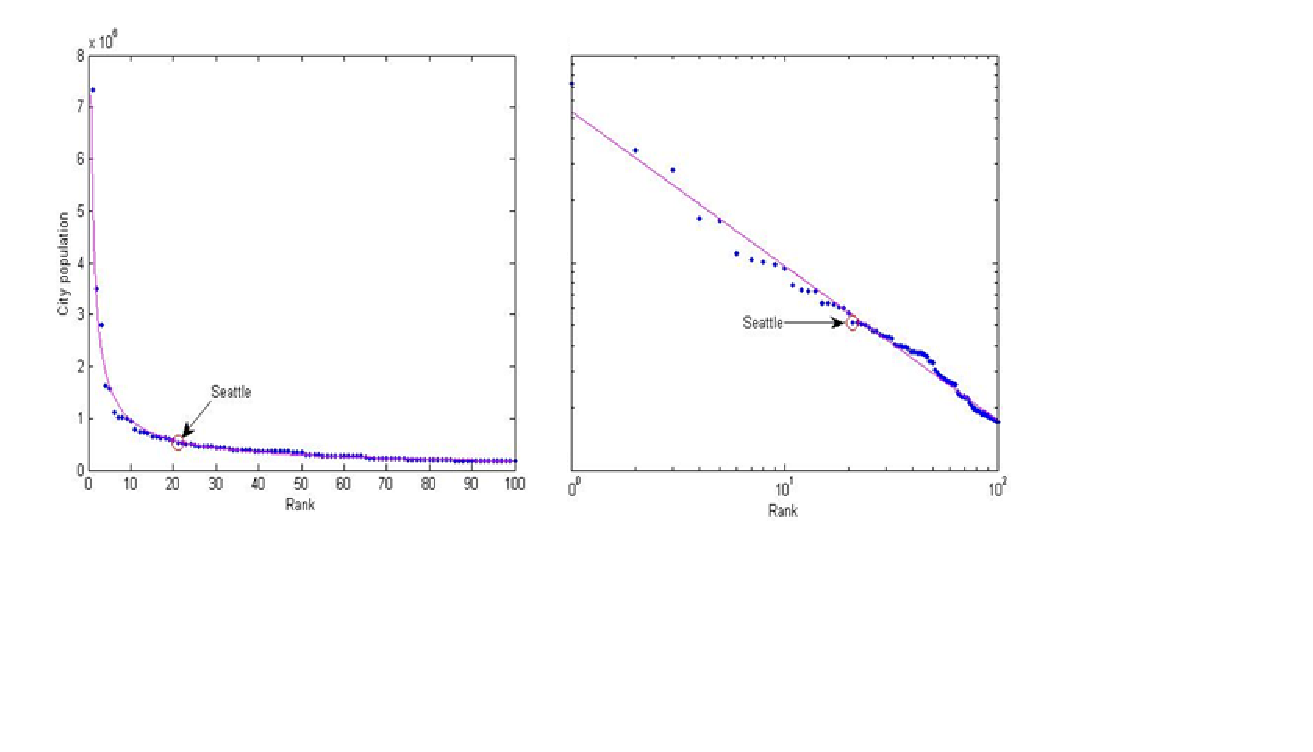
\includegraphics[scale=0.6]{Chapter1/PLgraph.eps}
\caption{City Population Graph}
\end{figure}

Important Observations:
\begin{enumerate}
\item The above graph follows power law distribution in its long-tail.
\item There are only few cities with very high population. There are more number of cities with less population
\item More people have moved from cities with low population to the cities with already high population
\item The rich-become-richer mechanism can be observed.
\end{enumerate}


% ------------------------------------------------------------------------


%%% Local Variables: 
%%% mode: latex
%%% TeX-master: "../thesis"
%%% End: 

%% Chapter2 has System Analysis and Design
\chapter{System Analysis and Design}
\ifpdf
    \graphicspath{{Chapter2/Chapter2Figs/PNG/}{Chapter2/Chapter2Figs/PDF/}{Chapter2/Chapter2Figs/}}
\else
    \graphicspath{{Chapter2/Chapter2Figs/EPS/}{Chapter2/Chapter2Figs/}}
\fi


All of the computations and graphics in this project are implemented using the Open Source statistical software R.\cite{R-cite}

\section{Introduction to R}

R is a free software programming language and software environment for statistical computing and graphics.
It is an implementation of the S programming language combined with lexical scoping semantics inspired by Scheme.
S was created by John Chambers while at Bell Labs. R was created by Ross Ihaka and Robert Gentleman
at the University Of Auckland, New Zealand, and is currently developed by the R Development Core Team.
R is a GNU project. The source code for the R software environment is written primarily in C, FORTRAN, and R.

R is especially suited to implement the statistical methods needed for network analysis. It provides a wide
variety of statistical and graphical techniques, including linear and nonlinear modelling, classical statistical tests,
time-series analysis, classification, clustering. Further, it is easily extensible through functions and extensions,
and the R community is noted for its active contributions in terms of packages.
Many of R’s standard functions are written in R itself, which makes it easy for users to follow the algorithmic choices made.
For computationally intensive tasks, C, C++, and FORTRAN code can be linked and called at run time.

\noindent {\bf The R Environment}

R is an integrated suite of software facilities for data manipulation, calculation and graphical display. Among other things it has
\begin{itemize}
\item An effective data handling and storage facility,
\item A suite of operators for calculations on arrays, in particular matrices,
\item A large, coherent, integrated collection of intermediate tools for data analysis, graphical facilities for data analysis and display either directly at the computer or on hard- copy, and
\item A well developed, simple and effective programming language which includes conditionals, loops, user defined recursive functions and input and output facilities.
\end{itemize}

R can be used as an environment within which many classical and modern statistical techniques have been implemented.
A few of these are built into the base R environment, but many are supplied as packages. There are about 25 packages
supplied with R (called standard and recommended packages) and many more are available through the CRAN family of
Internet sites (via http://CRAN.R-project.org).

All R functions and datasets are stored in packages. Only when a package is loaded are its contents available.
This is done both for efficiency (the full list would take more memory and would take longer to search than a subset),
and to aid package developers, who are protected from name clashes with other code.
Some of the R packages used in this project are Igraph, statnet, sna, ProNet and ergm.


% ------------------------------------------------------------------------

%%% Local Variables: 
%%% mode: latex
%%% TeX-master: "../thesis"
%%% End: 

%% Chapter3 has Results and Graphs
%\chapter{Analysis and Results}
\ifpdf
    \graphicspath{{Chapter3/Chapter3Figs/PNG/}{Chapter3/Chapter3Figs/PDF/}{Chapter3/Chapter3Figs/}}
\else
    \graphicspath{{Chapter3/Chapter3Figs/EPS/}{Chapter3/Chapter3Figs/}}
\fi

\section{Weight Assignment}
 
Considered here is a dataset consisting of email communications between a large network of individuals. For each email communication, information on sender(from) and receiver(to) is available. From this information, scores for edges are computed based on similarity feature and the score is associated with each edge to obtain the final weight.
Listed in the table given below are 10 of the total 59835 edges along with their corresponding weights.
  
\begin{table}[htb]
\caption{Weights for edges}
\begin{tabular}{ccl}\hline
from & to & weight\\ \hline
1 & 2 & 0.0315\\
3 & 4 & 0.0315\\
5 & 2 & 0.0315\\
6 & 7 & 0.0315\\
8 & 7 & 0.0315\\
9 & 10 & 0.0315\\
9 & 11 & 0.0315\\
12 & 13 & 0.0315\\
9 & 14 & 0.063\\
9 & 15 & 0.0315\\
\vdots&\vdots&\vdots\\ \hline
\end{tabular}\label{Table1}
\end{table}

\section{Influence Analysis}

For the network given in (\ref{Table1}) the clustering algorithm has identified 25 clusters. For each of these clusters, the scree plot is generated and the four approaches for influence analysis described in (\ref{SecIA}) are performed.
The results of this analysis for the first two clusters are shown in the figures given below.

\begin{figure}[htb]
\centering
\begin{minipage}{0.45\linewidth}
\includegraphics[scale=0.2]{Chapter3/Cluster_1_.eps}
\caption{Cluster 1}
\end{minipage}
\quad
\begin{minipage}{0.45\linewidth}
\includegraphics[scale=0.2]{Chapter3/Cluster_2_.eps}
\caption{Cluster 2}
\end{minipage}
\end{figure}
\pagebreak

\begin{figure}[htb]
\centering
\begin{minipage}{0.45\linewidth}
\includegraphics[scale=0.2]{Chapter3/Screeplot1_.eps}
\caption{Scree Plot 1}
\end{minipage}
\quad
\begin{minipage}{0.45\linewidth}
\includegraphics[scale=0.2]{Chapter3/Screeplot2_.eps}
\caption{Scree Plot 2}
\end{minipage}
\end{figure}
\pagebreak

\begin{figure}[htb]
\centering
\begin{minipage}{0.45\linewidth}
\includegraphics[scale=0.15]{Chapter3/AbsCut1_.eps}
\caption{Absolute cut score for cluster 1}
\end{minipage}
\quad
\begin{minipage}{0.45\linewidth}
\includegraphics[scale=0.15]{Chapter3/AbsCut2_.eps}
\caption{Absolute cut score for cluster 2}
\end{minipage}
\end{figure}

\begin{figure}[htb]
\centering
\begin{minipage}{0.45\linewidth}
\includegraphics[scale=0.15]{Chapter3/FixCut1_.eps}
\caption{Fixed percentage of population for cluster 1}
\end{minipage}
\quad
\begin{minipage}{0.45\linewidth}
\includegraphics[scale=0.15]{Chapter3/FixCut2_.eps}
\caption{Fixed percentage of population for cluster 2}
\end{minipage}
\end{figure}
\pagebreak

\begin{figure}[htb]
\centering
\begin{minipage}{0.45\linewidth}
\includegraphics[scale=0.15]{Chapter3/SdCut1_.eps}
\caption{Standard deviation for cluster 1}
\end{minipage}
\quad
\begin{minipage}{0.45\linewidth}
\includegraphics[scale=0.15]{Chapter3/SdCut2_.eps}
\caption{Standard deviation for cluster 2}
\end{minipage}
\end{figure}

\begin{figure}[htb]
\centering
\begin{minipage}{0.45\linewidth}
\includegraphics[scale=0.15]{Chapter3/RandomHist1_.eps}
\caption{Random Permutation Histogram for cluster 1}
\end{minipage}
\quad
\begin{minipage}{0.45\linewidth}
\includegraphics[scale=0.15]{Chapter3/RandomHist2_.eps}
\caption{Random Permutation Histogram for cluster 2}
\end{minipage}
\end{figure}
\pagebreak

\begin{figure}[htb]
\centering
\begin{minipage}{0.45\linewidth}
\includegraphics[scale=0.15]{Chapter3/RandomPlot1_.eps}
\caption{Random Permutation for cluster 1}
\end{minipage}
\quad
\begin{minipage}{0.45\linewidth}
\includegraphics[scale=0.15]{Chapter3/RandomPlot2_.eps}
\caption{Random Permutation for cluster 2}
\end{minipage}
\end{figure}

\section{Link Prediction}
 
For the network given in (\ref{Table1}) the probability of existence of an edge between any pair of nodes is computed as given in (\ref{SecLP}).
The result of this analysis is shown in the table given below.
  
\begin{table}[htb]
\caption{Probabilities for edges}
\begin{tabular}{ccl}\hline
from & to & probability\\ \hline
11 & 14 & 0.07272727\\
11 & 15 & 0.07272727\\
14 & 11 & 0.07272727\\
14 & 15 & 0.07272727\\
15 & 11 & 0.07272727\\
15 & 14 & 0.07272727\\
11 & 13 & 0.04848485\\
11 & 44 & 0.04848485\\
11 & 66 & 0.04848485\\
13 & 11 & 0.04848485\\
\vdots&\vdots&\vdots\\ \hline
\end{tabular}\label{Table2}
\end{table}

\section{Time Series Analysis}

For a social media dataset collected over time, time series analysis is performed to try and explore how this network reacts over time and how it behaves with the addition of new users, or which users tend to interact among each other. 

\begin{figure}[hb]
\centering
\begin{minipage}{0.45\linewidth}
\includegraphics[scale=0.15]{Chapter3/example104.eps}
\caption{At first time instance}
\end{minipage}
\quad
\begin{minipage}{0.45\linewidth}
\includegraphics[scale=0.15]{Chapter3/example425.eps}
\caption{At second time instance}
\end{minipage}
\end{figure}
% ------------------------------------------------------------------------


6)  Testing, Results and Discussion

Unit testing practices have been deployed in order to test the functionality of the source code and its behaviour. We found methods in order to improve efficiency of the source code. The above problem statements were run for a variety of data-sets and thus the underlying results matched the training data-set and the testing data-sets hence establishing proof of concept. Integration testing was performed as many individual modules were integrated into a single script and was rigorously tested in order to obtain a fully functional system. Big-data paradigm was introduced and initialized to see if the concepts could function regardless of the size of the input data-set. Scalability testing was performed in order to enrich the user’s experience and to make sure that the concept could run under heavy load regardless of the input size.

Conclusion from results

We have established an agile, reliable, scalable and robust model that fulfils all the desired requirements and thus has qualified to be a fully sustainable model.

Results ( Snapshots ) (Pending)



%%% Local Variables: 
%%% mode: latex
%%% TeX-master: "../thesis"
%%% End: 

%\chapter{Software Testing }
\ifpdf
    \graphicspath{{Chapter4/Chapter4Figs/PNG/}{Chapter4/Chapter4Figs/PDF/}{Chapter4/Chapter4Figs/}}
\else
    \graphicspath{{Chapter4/Chapter4Figs/EPS/}{Chapter4/Chapter4Figs/}}
\fi



  
% ------------------------------------------------------------------------

%%% Local Variables: 
%%% mode: latex
%%% TeX-master: "../thesis"
%%% End: 

\chapter{Methodology, Implementation and Results}


\section{Datasets Available on Networks, and Datasets Used}

\noindent {\bf SourceForge}

SourceForge is a web-based source code repository. It acts as a centralized location for software developers
to control and manage free and open source software development. It was the first to offer that service for
free to open source projects. The website runs a version of SourceForge Enterprise Edition, forked from the
last open-source version available. As of July 2011, the SourceForge repository hosts more than 300,000 projects
and has more than 2 million registered users, although not all are active.

\noindent {\bf Sourceforge.net}

SourceForge.net is the world’s largest Open Source software development web site, with the largest repository
of Open Source code and applications available on the Internet. Owned and operated by OSTG Inc. (``OSTG''),
SourceForge.net provides free services to Open Source developers. The SourceForge.net web site is database
driven and the supporting database includes historic and status statistics on over 100,000 projects and
over 1 million registered users’ activities at the project management web site. OSTG has shared certain
SourceForge.net data with the University of Notre Dame for the sole purpose of supporting academic and
scholarly research on the Free/Open Source Software phenomenon. OSTG has given Notre Dame permission to
in turn share this data with other academic researchers studying the Free/Open Source Software phenomenon.

\noindent {\bf Available Data}

SourceForge.net uses relational databases to store project management activity and statistics. There are over
100 relations (tables) in the monthly data dumps provided to Notre Dame. As of November 2005, the data warehouse was
almost 300 GB in size, and is growing at about 25 GB per month. Much of the data is duplicated among the monthly dumps,
but trends or changes in project activity and structure can be discovered by comparing data from the monthly dumps.
Queries across the monthly schema may be used to discover when changes took place, to estimate trends in project
activity and participation, or even that no activity, events or changes have taken place. To help researchers
determine what data is available, an ER-diagram and the definitions of tables and views in the data warehouse are provided.
For each month, the data warehouse includes three major parts:
\begin{itemize}
\item The tables supporting the SourceForge.net web site, for example, the tables user, group etc..
\item The tables used to store the statistics of the whole community, including daily page access, downloads etc.
\item The tables with the history information on the other tables.
\end{itemize}

\noindent {\bf Types of Data Used}

The following are the types of data that have been extracted from the SourceForge.net Research Data Archive for
the use in our project:
\begin{itemize}
\item Project sizes over time (number of developers as a function of time presented as a frequency distribution)
\item Development participation on projects (number of projects individual developers participate on presented as a frequency distribution)
\item Date of project creation (at SourceForge.net)
\item Date of first software release for a project
\item SourceForge.net ranking of projects at various times
\item Activity statistics on projects at various times
\item Number of projects in various software categories, e.g., games, communications, database, security, etc. Since all of the archived data is stored in a relational database, data to support FOSS investigations will be extracted using SQL queries against the data warehouse.
\end{itemize}
The first two items mentioned were used to create a ``collaboration social-network”, and also
to discover scale-free distributions among developer activity and project activity.

\section{Methods and Techniques}

\subsection{Weight Assignment}

\noindent {\bf Problem statement:}
Assign weights to an unweighted network dataset to obtain a clear and complete view of the network.

\noindent {\bf Dataset Used:}
\begin{enumerate}
\item {\em Co-authorship data}: This dataset contains authors where they are represented by the unique author's ID's.
A relation exist between two author ID's only if both have coauthored a book. Each author can be involved
in writing more than one book. In the graph format authors are represented by nodes or vertices and the
relations between them are represented by the presence of edge between them.
This is an undirected graph having 757 vertices and 1000 edges. 

\item {\em Email Communication Data}: This dataset contains the IDs of individuals who are actively involved
in a communication network via email. A relation between two IDs exist if any one of the two individuals
communicate through email. In the graph format, individuals are represented by nodes or vertices and the
relations between them are represented by the presence of edge between them. This is a directed graph having 1133 vertices and 10903 edges.
\end{enumerate}

\noindent {\bf Pseudocode/Algorithm}

\noindent Data : Unweighted RawDataFrame\\
\noindent Result : Weighted data

\begin{itemize}
\item Step 1 : Convert the data frame into graphs . Directed or undirected based on the data.
\item Step 2 : Remove all self loops and repeated edges.
\item Step 3 : Compute the similarity score using the intrinsic graph attributes.
\item Step 4 : Determine the weights from the similarity score.
\item Step 5 : Assign weights to each edge of the graph.
\item Step 6 : Generate weighted data file.
\end{itemize}

\noindent {\bf Procedure}

Given an unweighted social network dataset, it is possible to convert it into a weighted datagraph by
considering the features which are intrinsic to the graph. This process is performed using R software
which is a data mining tool for Big data as described previously. Further, R packages such as igraph,
sna, linkcomm and network, which again have been mentioned earlier, are used. Initially, a feature-rich
social network data is collected. It is converted into graphs. Outliers like self loops and repeated edges
are removed. A similarity score is calculated from a formula devised by taking into account the network
attributes and their definitions depending upon the data. Weights are computed from the score and are
assigned to each edge of the graph. Finally, these weights are appended to the input data and a new weighted dataset file is created.  

%\pagebreak
\noindent {\bf Results}

Results of the analysis are shown in Tables 4.1 and 4.2.

\begin{table}
\centering
\begin{tabular}{rr}\\ \hline
\multicolumn{2}{c}{Input}\\ \hline
FromNodeId &     ToNodeId\\ \hline
84424   & 276  \\
84424   & 1662 \\
84424   & 5089 \\
84424	& 6058 \\
84424	& 6229 \\
84424	& 10639 \\
84424	& 16442 \\
84424	& 19325 \\
84424	& 19834 \\
84424	& 20113 \\
84424	& 21937 \\
\vdots  & \vdots \\ \hline
\end{tabular}\\
\begin{tabular}{rrr}\\ \hline
\multicolumn{3}{c}{Output}\\ \hline
FromNodeId &     ToNodeId & Weight\\ \hline
84424   & 276  & 0.1549\\
84424   & 1662 & 0.1549\\
84424   & 5089 & 0.1549\\
84424   & 6058 & 0.1549\\
84424   & 6229 & 0.1549\\
84424   & 10639 & 0.0684\\
84424   & 16442 & 0.0684\\
84424   & 19325 & 0.0684\\
84424   & 19834 & 0.0684\\
84424   & 20113 & 0.0684\\
84424   & 21937 & 0.0684\\
\vdots  & \vdots & \vdots\\ \hline
\end{tabular}\\
\caption{Co-authorship Data}
\end{table}


\begin{table}
\centering
\begin{tabular}{rr}\\ \hline
\multicolumn{2}{c}{Input}\\ \hline
FromNodeId &     ToNodeId \\ \hline
1          &  2  \\
1          &  3  \\
1          &  4  \\
1          &  5  \\
1          &  6  \\
1          &  7  \\
1          &  8  \\
1          &  9  \\
1          &  10  \\
1          &  11  \\
\vdots & \vdots \\ \hline
\end{tabular}\\
\begin{tabular}{rrr}\\ \hline
\multicolumn{3}{c}{Output}\\ \hline
FromNodeId &     ToNodeId & Weight\\ \hline
1          &  2  & 0.0928\\
1          &  3  & 0.1194\\
1          &  4  & 0.0911\\
1          &  5  & 0.0698\\
1          &  6  & 0.0893\\
1          &  7  & 0.0981\\
1          &  8  & 0.0663\\
1          &  9  & 0.0822\\
1          &  10  & 0.1088\\
1          &  11  & 0.0875\\
\vdots & \vdots & \vdots\\ \hline
\end{tabular}
\caption{Email Communication Data}
\end{table}

\pagebreak
\subsection{Sampling Based Influence Analysis for Large Networks}

\noindent {\bf Problem statement:} Given a network of a very large size conduct
influence analysis on it.

\noindent {\bf Dataset Used:}\\
{\em January 2009 SourceForge data}: This dataset contains developers where they are represented by the unique developer's ID's.
A relation exists between two developer ID's only if both have collaborated on a project. Each developer can be involved
in developing multiple projects. In the graph format developers are represented by nodes or vertices and the
relations between them are represented by the presence of edge between them.
This is a directed graph having 36111 vertices and 209491 edges.

\noindent {\bf Method}

The standard techniques for clustering fail when one applies them to very large
networks due to computational complexity. The alternative suggested here is to
identify the major subnetworks of such a large network first, and then to
conduct influence analysis for each of the large subnetworks. The question is
how one can identify the clusters within a network without a complete exploration
of the entire network. Here is where probabilistic methods help. Probability
theory, especially the Law of Large Numbers, says that under general conditions,
random sampling can be used to identify important features of a population.
Consider a large network to be a given population and apply random sampling
to extract a sample. Treat this as a randomly generated subnetwork. As long
as the sample size is reasonable, clustering algorithms will work efficiently
on the sampled subnetwork. Now apply the Law of Large Numbers and claim
that if the sampling is continued, then sooner or later, the nature of
clusters within the large network will emerge. Consequently, the influence
analysis conducted on a reasonable sized random subnetwork will closely
approximate the influence analysis of the entire network. One just needs
to continue sampling until the number of clusters obtained stabilizes.

\pagebreak
\noindent {\bf Pseudocode/Algorithm}

\noindent Data : Network Data\\
\noindent Result : Large Subnetworks, Influential nodes

\begin{itemize}
\item Step 1 :  Convert the network into a graph where $N$ is the total number of vertices,
directed or undirected based on the data.
\item Step 2 :  Initialize the sample size to $n$ = 10\% of $N$.
Sample a subnetwork consisting of $n$ vertices.
\item Step 3 : Apply the Fast Greedy clustering algorithm to the sampled subnetwork and
obtain the clusters therein. Drop all clusters of size less than 1\% of $n$.
\item Step 4 : Check whether the stopping rule (*) is satisfied. If yes, go to Step 6;
else go to Step 5.
\item Step 5 : Increment $n$ by 10\% (of $N$) and repeat Steps 2 and 3.
\item Step 6 : Complete the clustering of the entire network by assigning the unsampled
vertices to the identified clusters using the PageRank algorithm.
\item Step 7 : Perform influence analysis on each of the finally obtained clusters.
\end{itemize}
(*): The stopping rule used in this project is as follows: Let $a_i$ be the number of clusters
obtained in the $i$th iteration. Define $b_i = |a_{i+1}-a_i|$ and $c_i = |b_{i+1}-b_i|$. Stop
when $c_{i+1}\le c_i$.

\noindent {\bf Procedure}

Given a large social network dataset, it is possible to identify the influential individuals
by performing influence analysis on this network.
This approach is implemented using R software which is a statistical programming language.
R packages such as igraph, sna, network, ProNet and ergm are used. Initially, a feature-rich
social network data is collected. It is converted into graphs. Outliers like self loops and repeated edges
are removed. Subnetworks of increasingly large sample sizes are randomly extracted and
clustered. Once this stabilizes, the unsampled vertices are assigned to the obtained large
subnetworks using PageRank. Subsequently, influence analysis is performed on the identified clusters.

\noindent {\bf Results}

Results of the analysis are shown in Tables 4.3 and 4.4, and Figures 4.1 - 4.18.

\begin{table}
\centering
\begin{tabular}{rr}\\ \hline
\multicolumn{2}{c}{Input}\\ \hline
From & To\\ \hline
0 & 28234 \\
0 & 9031 \\
1 & 27082 \\
1 & 23805 \\
1 & 21702 \\
1 & 35191 \\
1 & 22520 \\
1 & 28220 \\
1 & 36 \\
\vdots & \vdots \\ \hline
\end{tabular}
\caption{January 2009 SourceForge Data}
\end{table}

\begin{table}
\centering
\begin{tabular}{rrr}\\ \hline
Sample percent & Number of vertices selected & Number of clusters found\\ \hline
10 & 3611 & 1\\
20 & 7222 & 5\\
30 & 10833 & 10\\
40 & 14444 & 10\\ \hline
\end{tabular}
\caption{Number of clusters versus sampling percentage}
\end{table}

\begin{figure}[htb]
\centering
\begin{minipage}{0.45\linewidth}
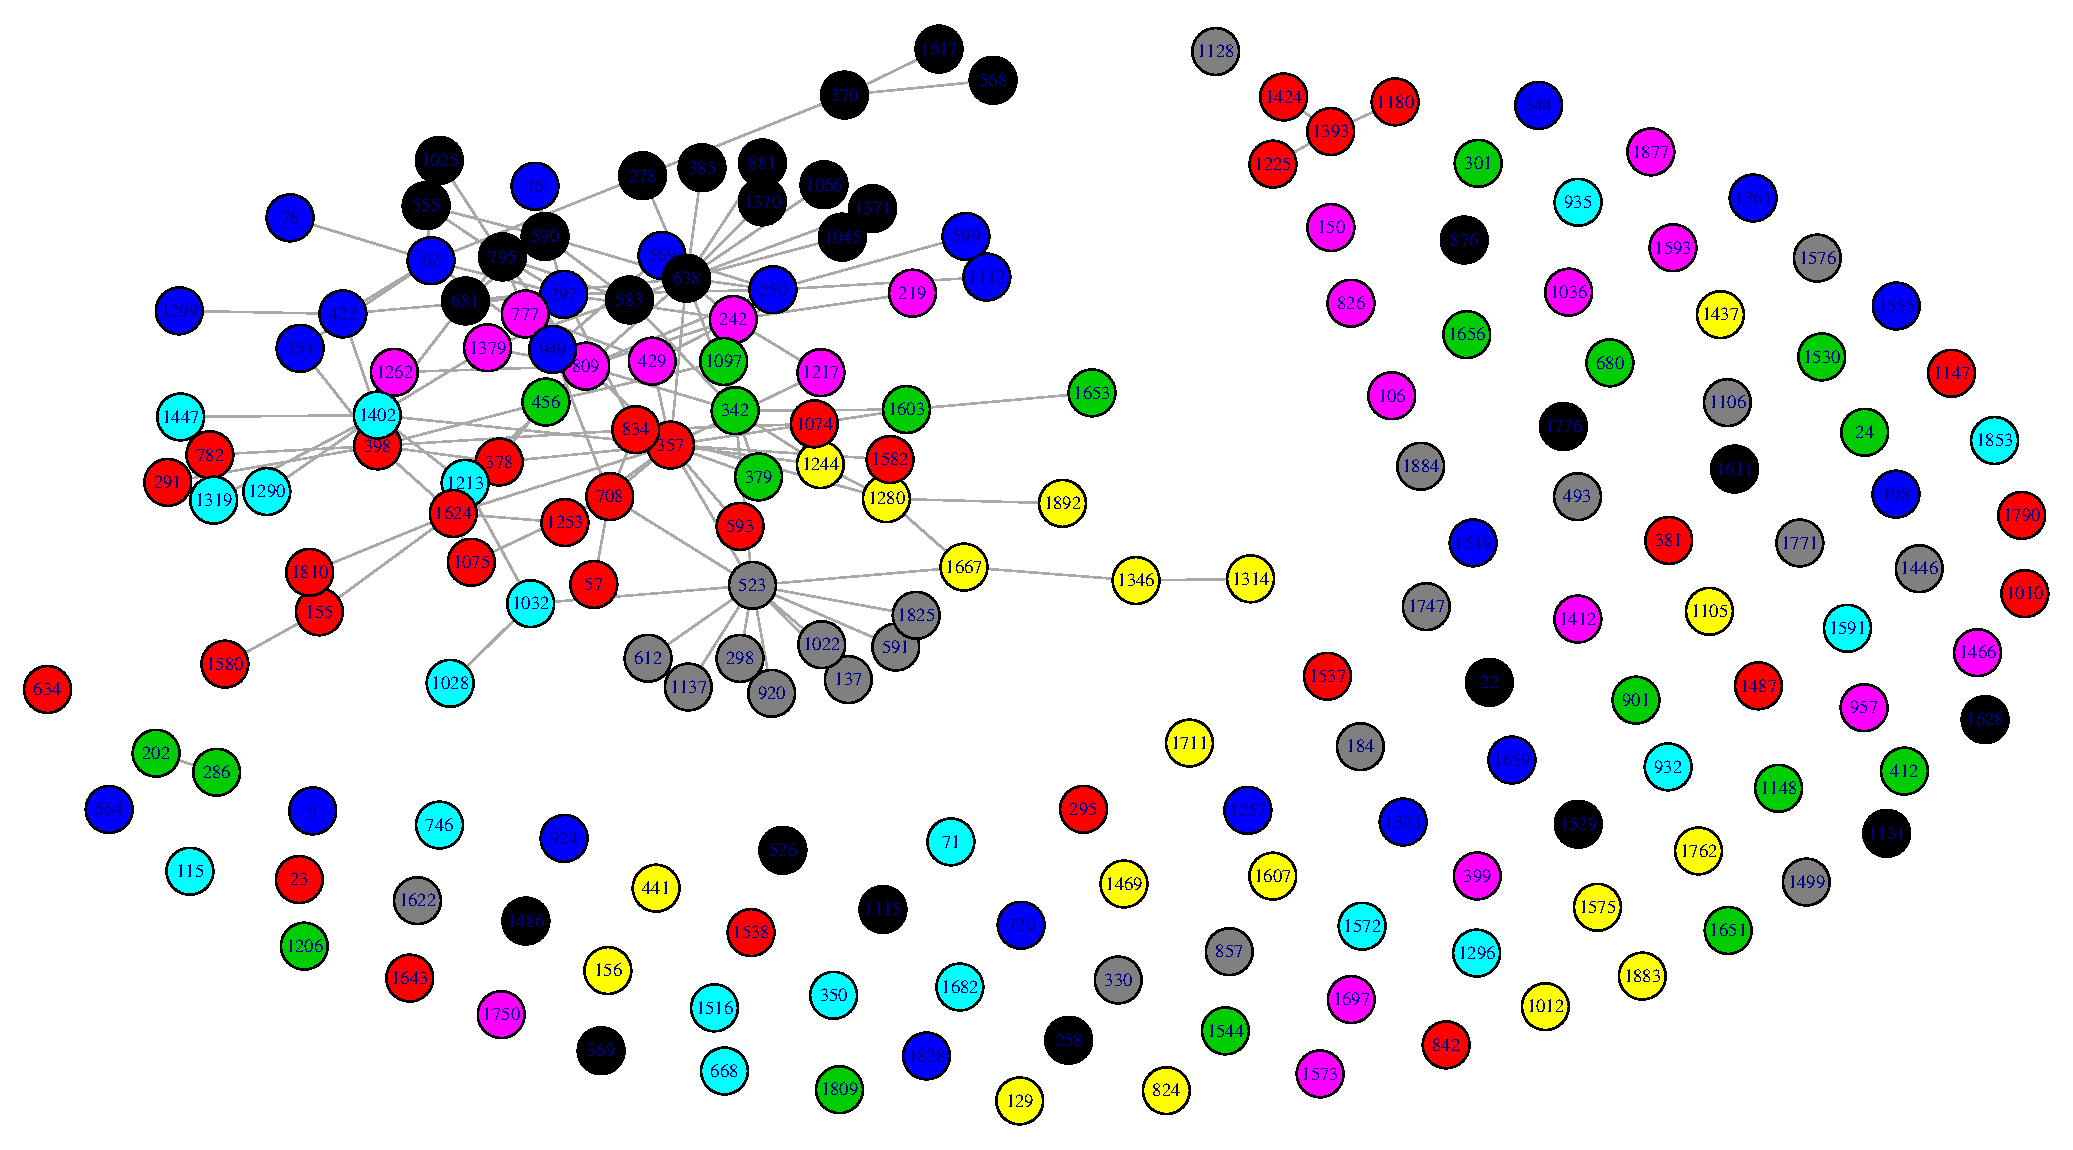
\includegraphics[scale=0.2]{Methods/10percent.eps}
\caption{Clusters with 10\% sampling}
\end{minipage}
\quad
\begin{minipage}{0.45\linewidth}
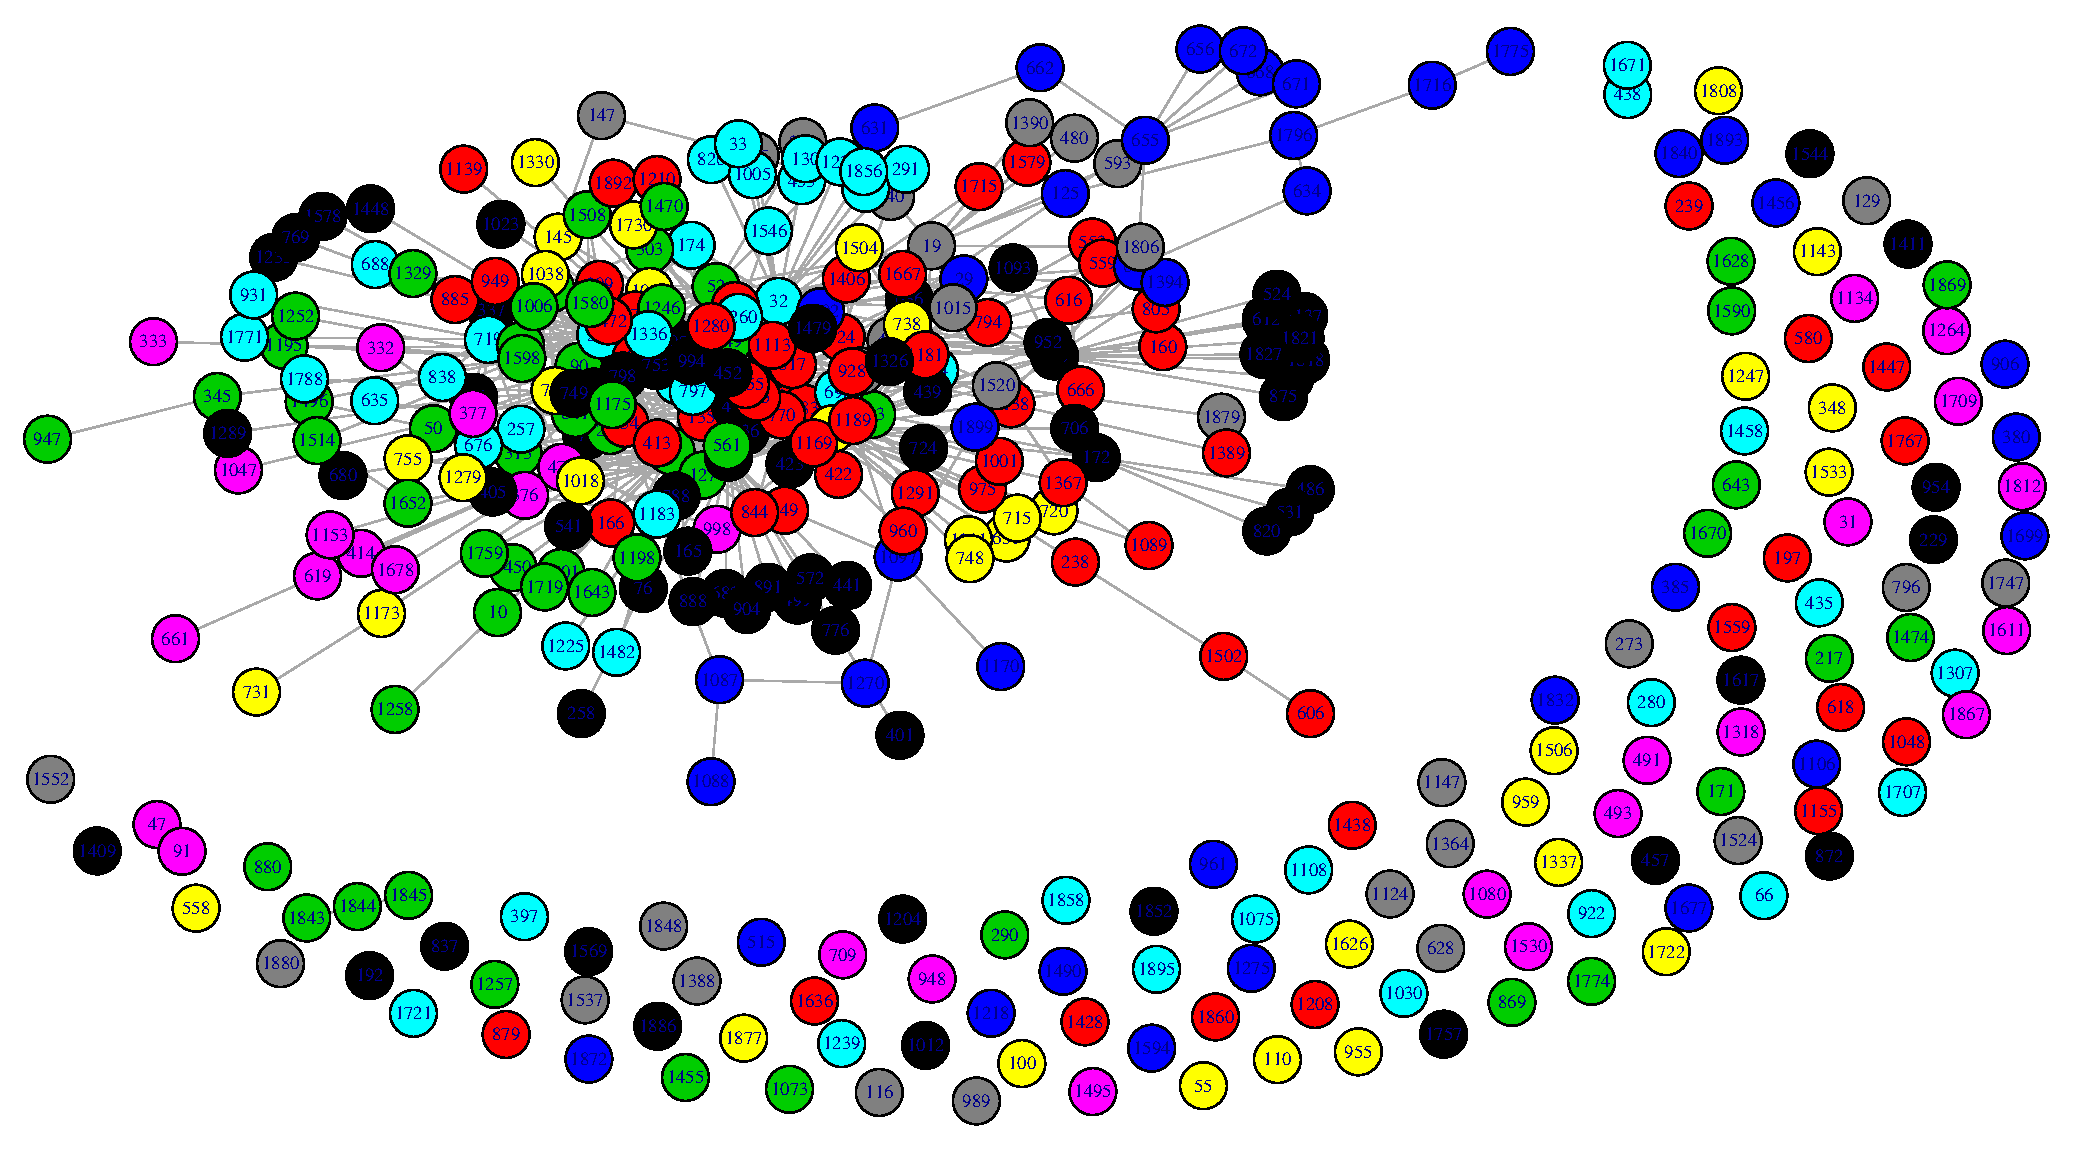
\includegraphics[scale=0.2]{Methods/20percent.eps}
\caption{Clusters with 20\% sampling}
\end{minipage}
\end{figure}
\pagebreak

\begin{figure}[htb]
\centering
\begin{minipage}{0.45\linewidth}
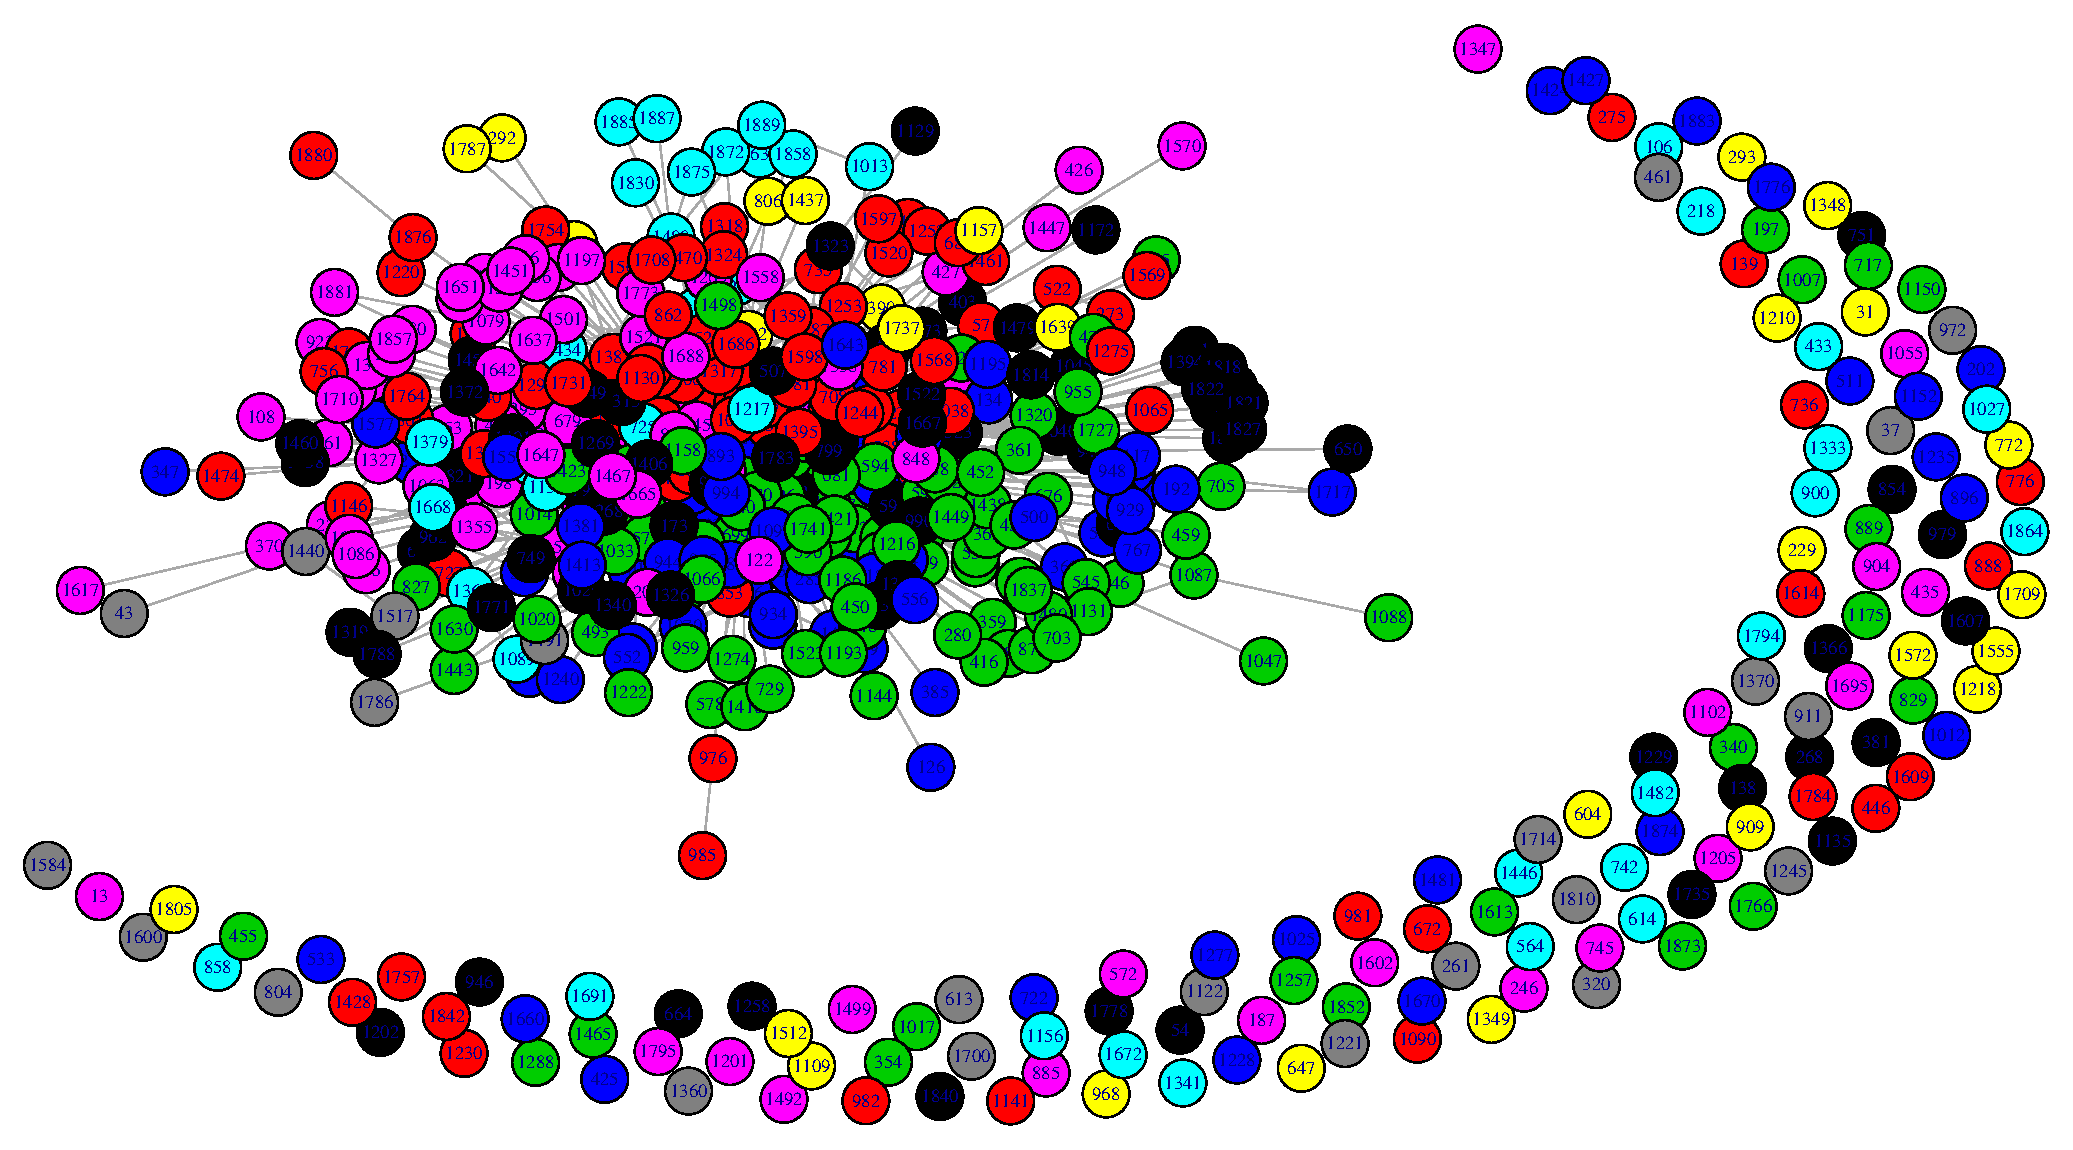
\includegraphics[scale=0.2]{Methods/30percent.eps}
\caption{Clusters with 30\% sampling}
\end{minipage}
\quad
\begin{minipage}{0.45\linewidth}
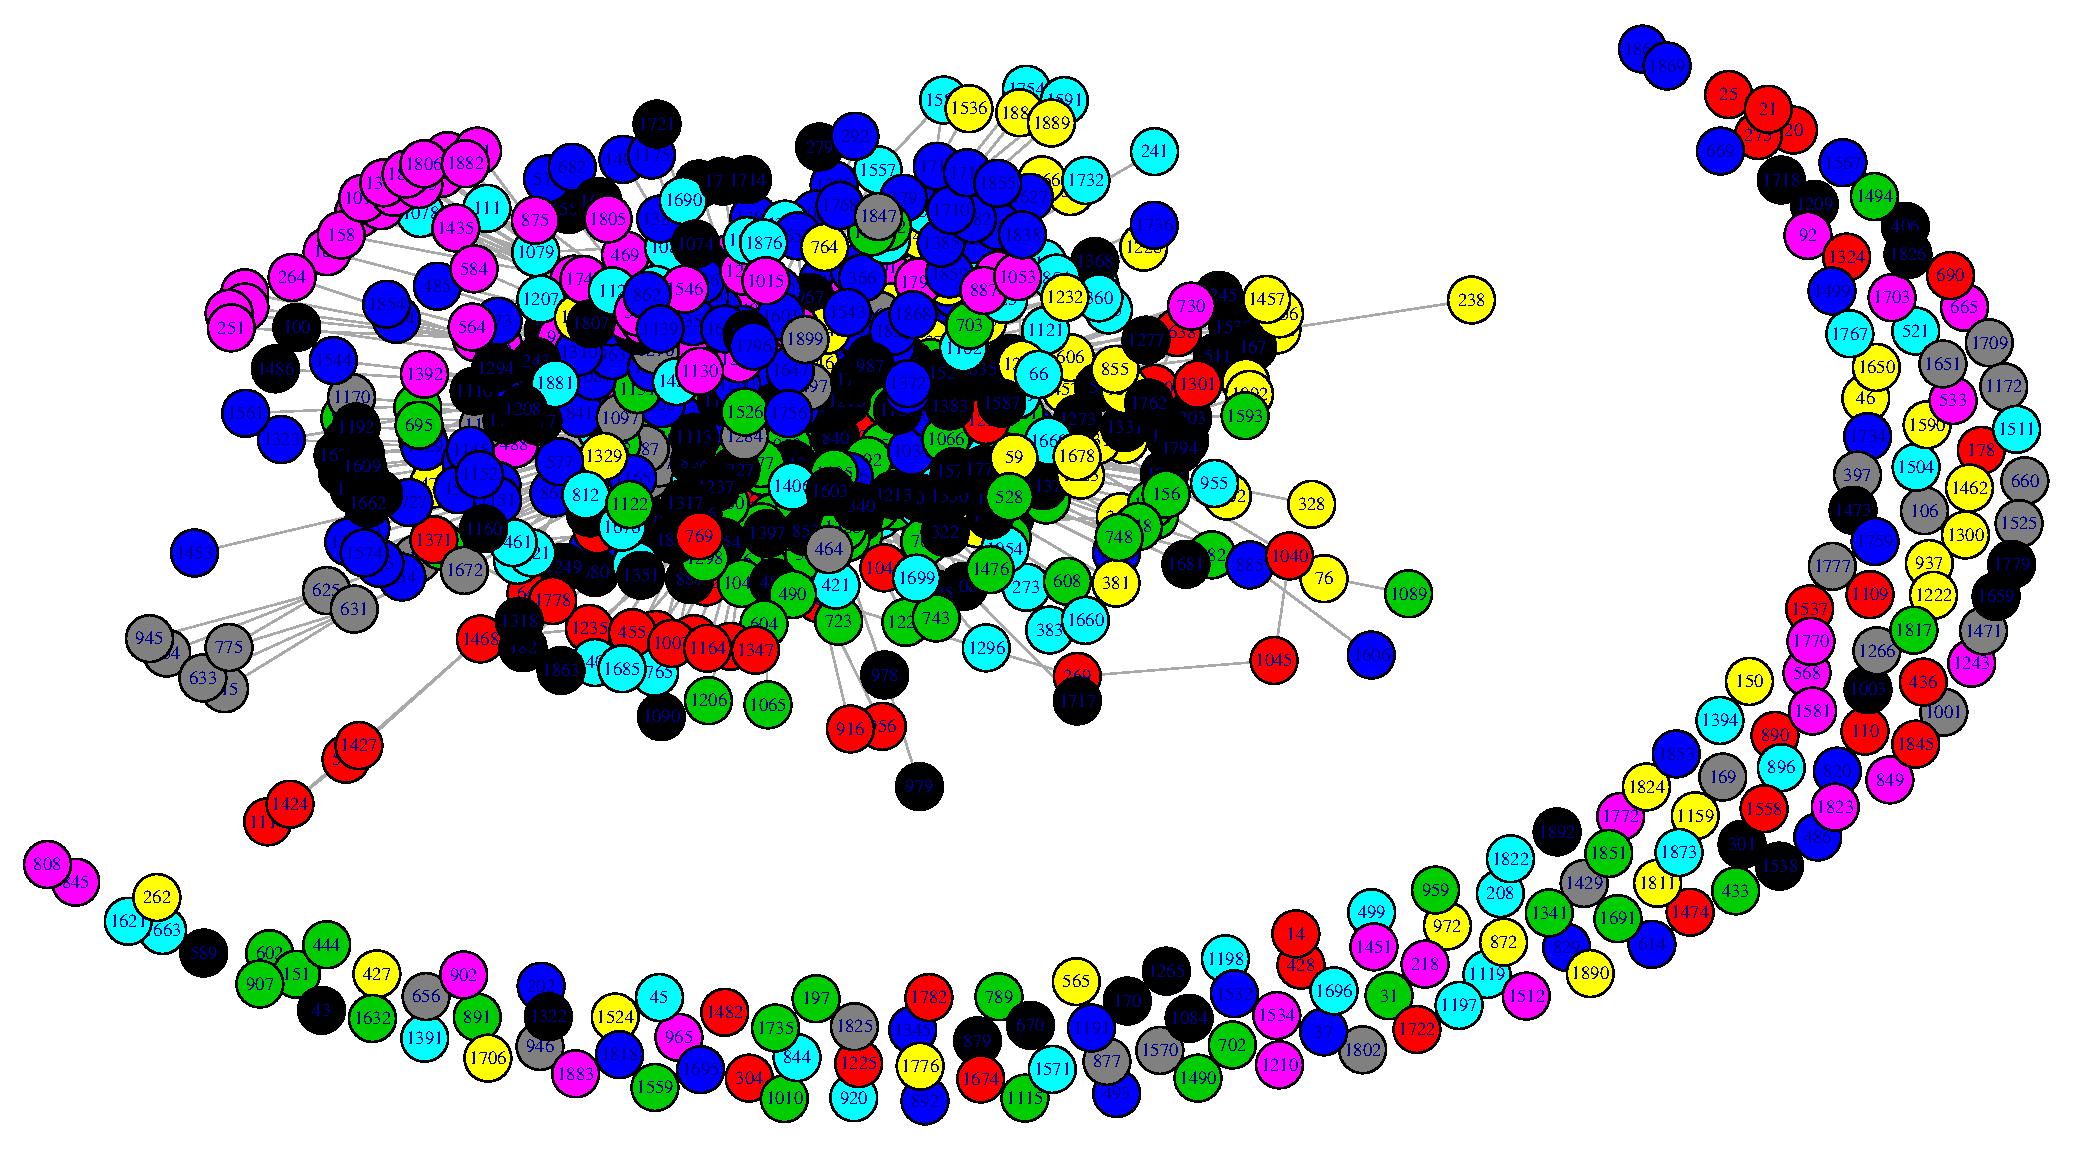
\includegraphics[scale=0.2]{Methods/40percent.eps}
\caption{Clusters with 40\% sampling}
\end{minipage}
\end{figure}
\pagebreak

\begin{figure}[htb]
\centering
\begin{minipage}{0.45\linewidth}
\includegraphics[scale=0.2]{Methods/Cluster_1_.eps}
\caption{Cluster 1}
\end{minipage}
\quad
\begin{minipage}{0.45\linewidth}
\includegraphics[scale=0.2]{Methods/Cluster_2_.eps}
\caption{Cluster 2}
\end{minipage}
\end{figure}
\pagebreak

\begin{figure}[htb]
\centering
\begin{minipage}{0.45\linewidth}
\includegraphics[scale=0.2]{Methods/Screeplot1_.eps}
\caption{Scree Plot 1}
\end{minipage}
\quad
\begin{minipage}{0.45\linewidth}
\includegraphics[scale=0.2]{Methods/Screeplot2_.eps}
\caption{Scree Plot 2}
\end{minipage}
\end{figure}
\pagebreak

\begin{figure}[htb]
\centering
\begin{minipage}{0.45\linewidth}
\includegraphics[scale=0.15]{Methods/AbsCut1_.eps}
\caption{Absolute cut score for cluster 1}
\end{minipage}
\quad
\begin{minipage}{0.45\linewidth}
\includegraphics[scale=0.15]{Methods/AbsCut2_.eps}
\caption{Absolute cut score for cluster 2}
\end{minipage}
\end{figure}

\begin{figure}[htb]
\centering
\begin{minipage}{0.45\linewidth}
\includegraphics[scale=0.15]{Methods/FixCut1_.eps}
\caption{Fixed percentage of population for cluster 1}
\end{minipage}
\quad
\begin{minipage}{0.45\linewidth}
\includegraphics[scale=0.15]{Methods/FixCut2_.eps}
\caption{Fixed percentage of population for cluster 2}
\end{minipage}
\end{figure}
\pagebreak

\begin{figure}[htb]
\centering
\begin{minipage}{0.45\linewidth}
\includegraphics[scale=0.15]{Methods/SdCut1_.eps}
\caption{Standard deviation for cluster 1}
\end{minipage}
\quad
\begin{minipage}{0.45\linewidth}
\includegraphics[scale=0.15]{Methods/SdCut2_.eps}
\caption{Standard deviation for cluster 2}
\end{minipage}
\end{figure}

\begin{figure}[htb]
\centering
\begin{minipage}{0.45\linewidth}
\includegraphics[scale=0.15]{Methods/RandomHist1_.eps}
\caption{Random Permutation Histogram for cluster 1}
\end{minipage}
\quad
\begin{minipage}{0.45\linewidth}
\includegraphics[scale=0.15]{Methods/RandomHist2_.eps}
\caption{Random Permutation Histogram for cluster 2}
\end{minipage}
\end{figure}
\pagebreak

\begin{figure}[htb]
\centering
\begin{minipage}{0.45\linewidth}
\includegraphics[scale=0.15]{Methods/RandomPlot1_.eps}
\caption{Random Permutation for cluster 1}
\end{minipage}
\quad
\begin{minipage}{0.45\linewidth}
\includegraphics[scale=0.15]{Methods/RandomPlot2_.eps}
\caption{Random Permutation for cluster 2}
\end{minipage}
\end{figure}

\subsection{Link Prediction}

\noindent {\bf Problem statement:} To apply efficient link prediction algorithms to uncover developer
relations and to predict future outcomes.

\noindent {\bf Dataset Used:}
\begin{enumerate}
\item {\em Co-authorship data}: This dataset contains authors where they are represented by the unique author's ID's.
A relation exists between two author ID's only if both have coauthored a book. Each author can be involved
in writing more than one book. In the graph format authors are represented by nodes or vertices and the
relations between them are represented by the presence of edge between them.
This is an undirected graph having 757 vertices and 1000 edges. 

\item {\em Email Communication Data}: This dataset contains the IDs of individuals who are actively involved
in a communication network via email. A relation between two IDs exist if any one of the two individuals
communicate through email. In the graph format, individuals are represented by nodes or vertices and the
relations between them are represented by the presence of edge between them. This is a directed graph having 1133 vertices and 10903 edges.
\end{enumerate}

\noindent {\bf Pseudocode/Algorithm}

\noindent Data : Weighted RawDataFrame\\
\noindent Result : Edges with corresponding similarity scores

\begin{itemize}
\item Step 1 : Convert the data frame into graphs . Directed or undirected based on the data.
\item Step 2 : Remove all self loops and repeated edges.
\item Step 3: Compute probabilities of existence and non-existence of any link in the graph
\item Step 4: Compute clusters using fast greedy approach
\item Step 5: Given a non existent link,
\begin{itemize}
\item a) Compute total number of common neighbours
\item b) Compute number of common neighbours within common groups
\item c) Determine from a) and b) the number of common neighbours outside of common groups
\end{itemize}
\item Step 6: Compute the similarity score
\item Step 7: Sort all the edges in the decreasing order of their similarity scores
\end{itemize}

\noindent {\bf Procedure}

Given a weighted social network dataset, link prediction can be performed by using the structural properties
of the network and community information of the nodes present in the network. This process is performed using
R software which is a data mining tool for Big data. R packages such as igraph, sna, proxy are used. A feature
rich, weighted social network dataset is taken as the input. It is converted into graph with no self loops and
repeated edges. To obtain community information of the nodes in the graph, a fast greedy algorithm is applied.
The probabilities of existence and non-existence of any link in the graph is computed. Now, given any non-existent link,
the number of common neighbours within and outside of common groups and the total number of common neighbours is computed.
Using the parameters computed above a similarity score is assigned to every non-existent link. All the links are sorted
in the decreasing order of their similarity score.

\noindent {\bf Results}

Results of the analysis are shown in Table 4.5.

\begin{table}[htb]
\centering
\begin{tabular}{ccl}\hline
from & to & probability\\ \hline
11 & 14 & 0.07272727\\
11 & 15 & 0.07272727\\
14 & 11 & 0.07272727\\
14 & 15 & 0.07272727\\
15 & 11 & 0.07272727\\
15 & 14 & 0.07272727\\
11 & 13 & 0.04848485\\
11 & 44 & 0.04848485\\
11 & 66 & 0.04848485\\
13 & 11 & 0.04848485\\
\vdots&\vdots&\vdots\\ \hline
\end{tabular}\label{Table2}
\caption{Probabilities for edges}
\end{table}


\subsection{Time Series Analysis}

\noindent {\bf Problem statement:}
Time Series Analysis provides us with a pragmatic view of the overall network with respect to time in a
dynamic fashion in order to understand the growth, evolution and the final outcome of the social network
by the effective use of time varying graphs and temporal indicator metrics.

\noindent {\bf Dataset Used:}
\begin{enumerate}
\item {\em Twitter data}: This dataset contains where twitter-user's the they are represented by the unique
twitter ID's. A relation exist between two twitter ID's only if both have had an interaction. The twitter
users having one or many interactions at any given time. In the graph theory paradigm twitter users are
represented by nodes or vertices and time used as a sole parameter to evaluate them.

\item {\em Source-Forge data}: This is a dataset which contains unique developer ID's and their interactions over time.
In the graph theory paradigm developers are represented by nodes or vertices and time used as a sole parameter to evaluate them.
\end{enumerate}

\noindent {\bf Pseudocode/Algorithm}

\noindent Result : Complete analysis and growth of the network over time.

\begin{itemize}
\item Step 1 : Load dataset with nodes, edges and time stamps.
\item Step 2 : Generate an initial sub-graph with a suitable colour pallete.
\item Step 3 : Generate subsequent layout using graphopt with normalized coordinates.
\item Step 4 : Determine a suitable time slot and generate other subgraphs illustrating growth.
\item Step 5 : Time loop starts and remove edges which are not present.
\item Step 6 : A final graph is obtained indicating all the interactions.
\item Step 7 : The most influential person in the network is determined.
\end{itemize}

\noindent {\bf Procedure}

A suitable twitter dataset has been analysed dynamically in order to understand the growth of the social network.
Temporal graph and time varying graph algorithms are rigorously implemented. It is of interest to understand the evolution
of the network and forecast the most influential entity. Snapshots of the subnetworks are generated periodically.
The final network shows interactions of all the individuals in the network. The following snapshots are clubbed into
flash content in order to get aesthetically stimulating result.

\noindent {\bf Results}

Results of the analysis are shown in Table 4.6 and Figures 4.19 - 4.21.

\begin{table}
\centering
\begin{tabular}{lll}\\ \hline
\multicolumn{3}{c}{Input}\\ \hline
id1 & id2 & time \\ \hline
1 & 2 & 1 \\
1 & 3 & 1 \\
2 & 3 & 1 \\
5 & 3 & 2 \\
6 & 2 & 3 \\
7 & 2 & 4 \\
8 & 7 & 5 \\
9 & 5 & 6 \\
10 & 7 & 7 \\
\vdots & \vdots &\vdots\\ \hline
\end{tabular}
\caption{Time Series Analysis of Twitter Data}
\end{table}

\begin{figure}[hb]
\centering
\begin{minipage}{0.45\linewidth}
\includegraphics[scale=0.15]{Methods/example104.eps}
\caption{At first time instance}
\end{minipage}
\quad
\begin{minipage}{0.45\linewidth}
\includegraphics[scale=0.15]{Methods/example425.eps}
\caption{At second time instance}
\end{minipage}
\end{figure}
\begin{figure}
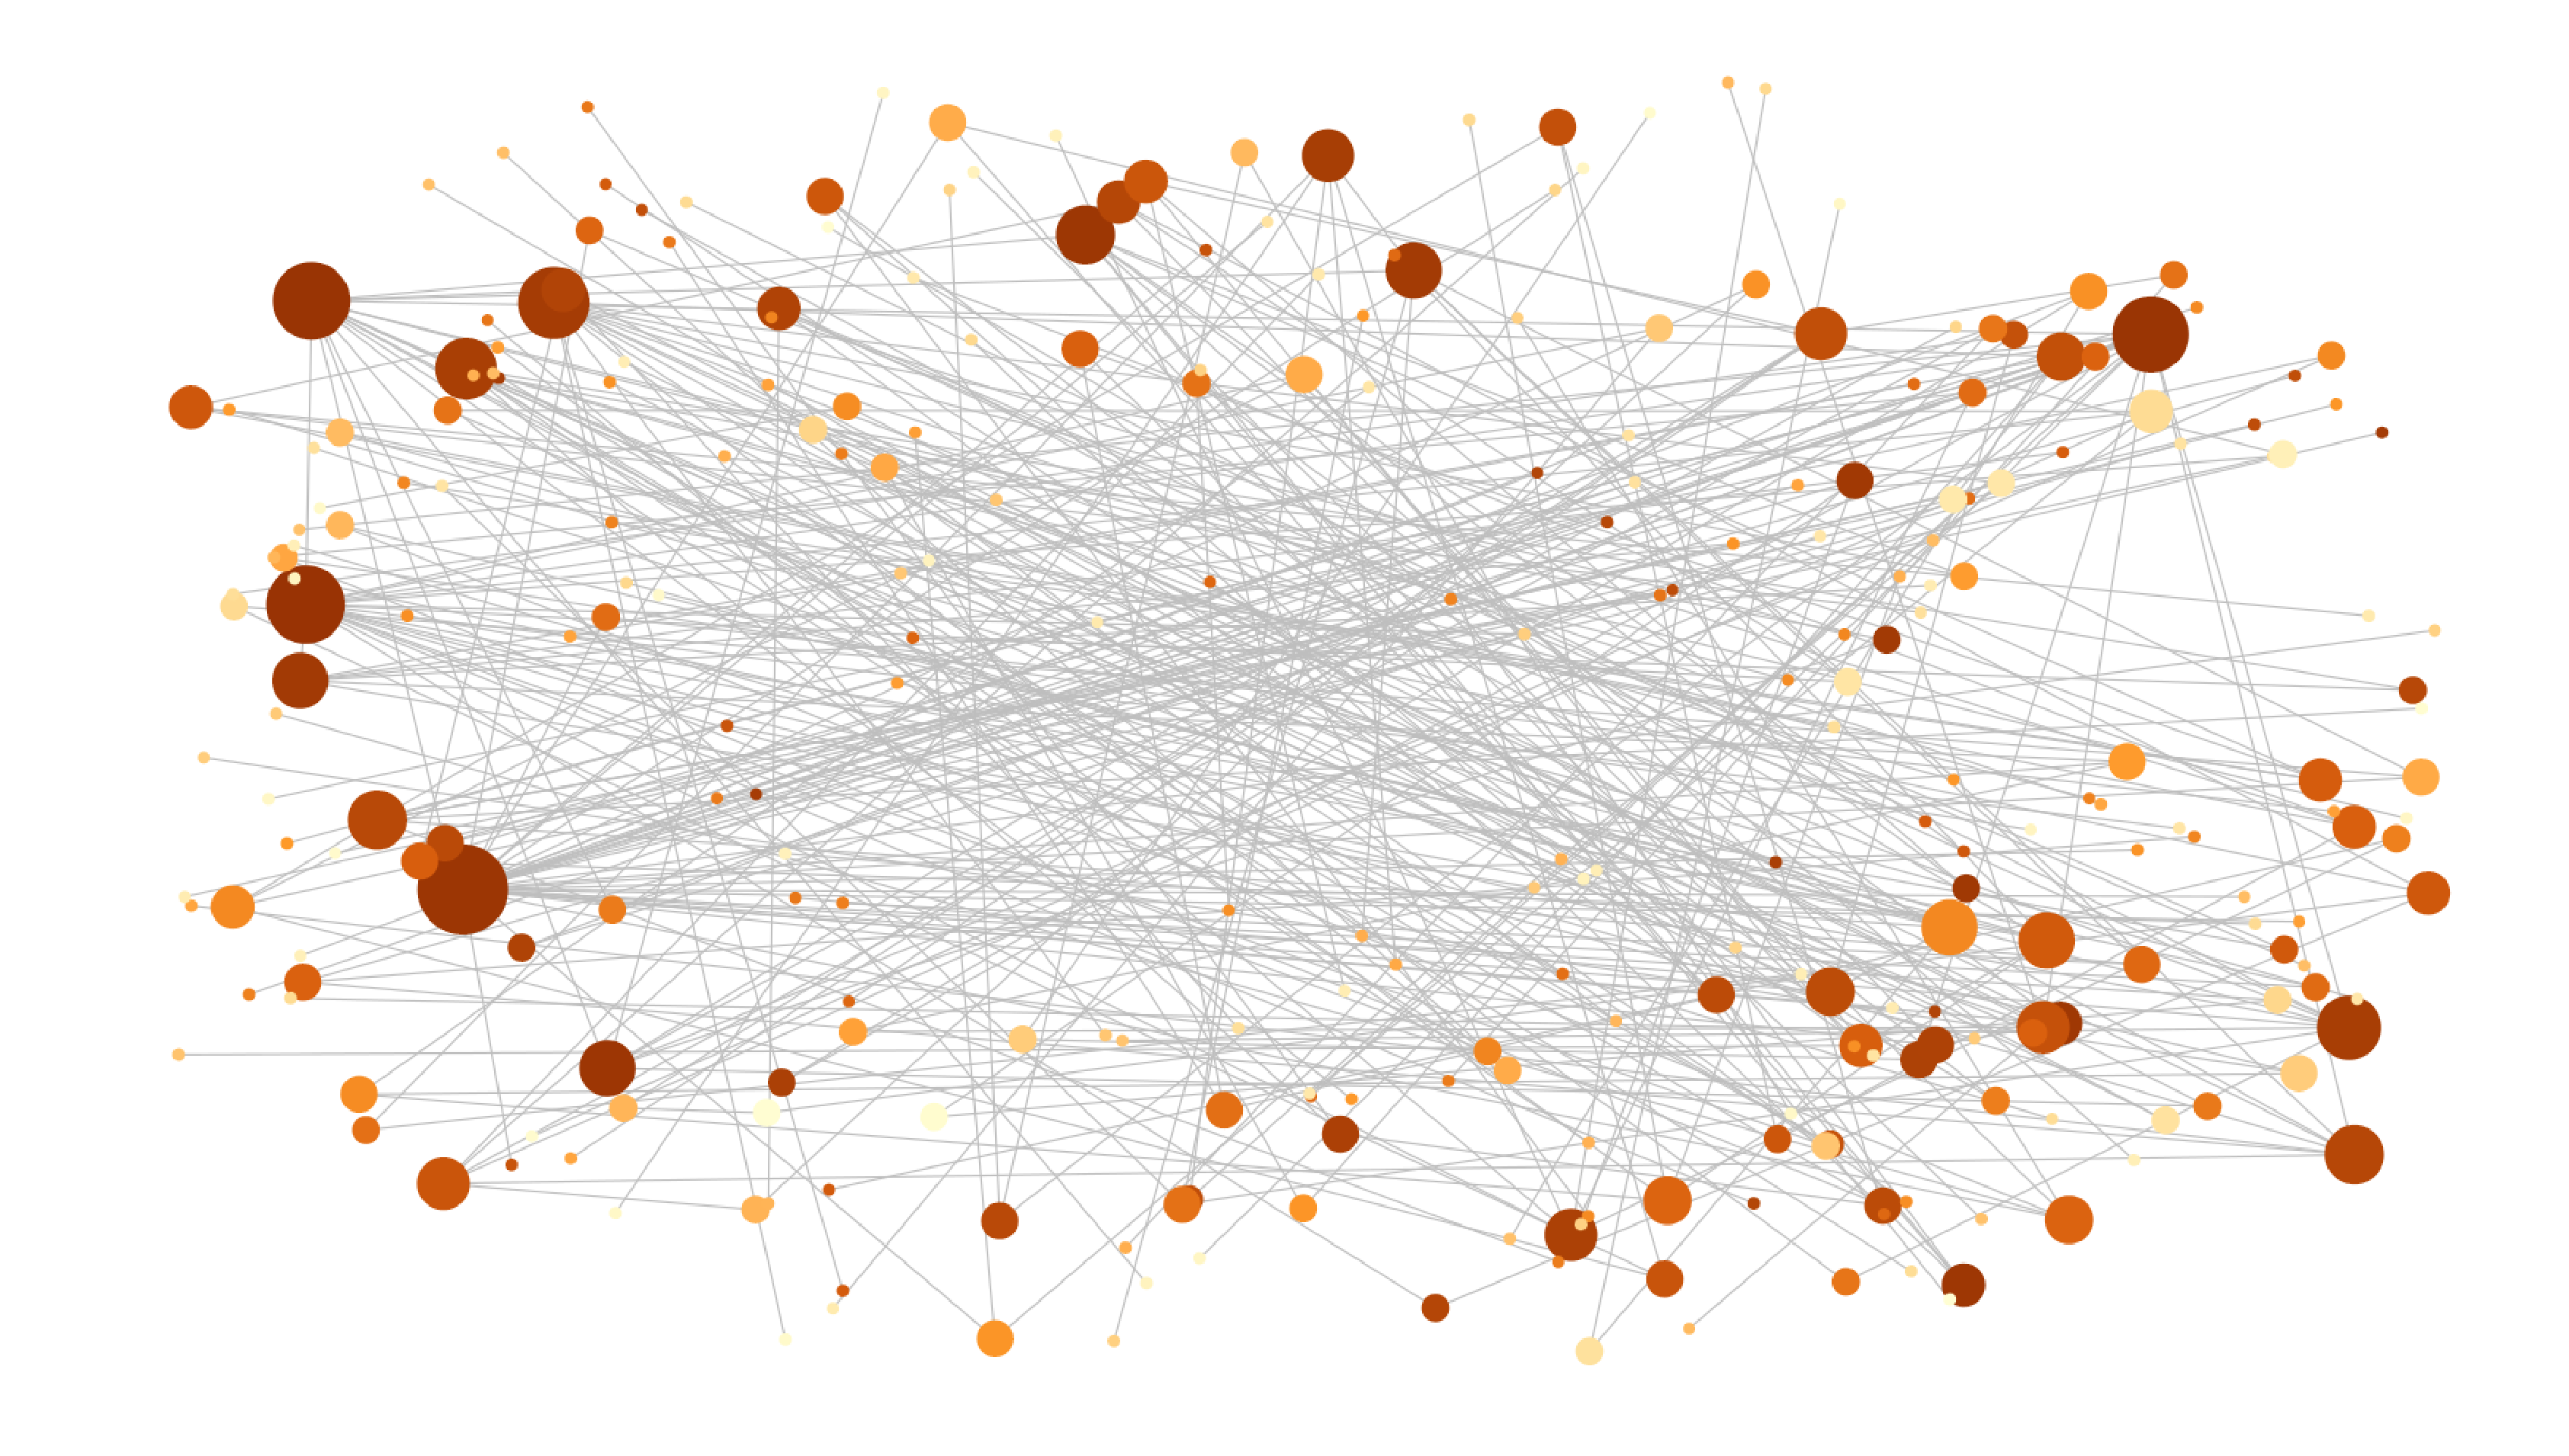
\includegraphics[scale=0.3]{Methods/example2971.eps}
\caption{At the final time instance}
\end{figure}

% ------------------------------------------------------------------------


%%% Local Variables:
%%% mode: latex
%%% TeX-master: "../thesis"
%%% End:



\def\baselinestretch{1}
\chapter{Testing, Conclusions and Future Work}
\ifpdf
    \graphicspath{{Conclusions/ConclusionsFigs/PNG/}{Conclusions/ConclusionsFigs/PDF/}{Conclusions/ConclusionsFigs/}}
\else
    \graphicspath{{Conclusions/ConclusionsFigs/EPS/}{Conclusions/ConclusionsFigs/}}
\fi

\def\baselinestretch{1.66}

\section{Testing}
Unit testing practices have been deployed in order to test the functionality of the source code and its behaviour. We found methods to improve efficiency of the source code. The above algorithms were run for a variety of data-sets and thus the underlying results matched the training data-set and the testing data-sets, thus establishing proof of concept. Integration testing was performed as many individual modules were integrated into a single script and was rigorously tested in order to obtain a fully functional system. Big-data paradigm was introduced and initialized to see if the concepts could function regardless of the size of the input data-set. Scalability testing was performed in order to enrich the user’s experience and to make sure that the concept could run under heavy load regardless of the input size.

\section{Conclusions}

Weights play an important role in the analysis of social networks. They represent the strength of interaction between the nodes. In this project, weights have been assigned to each edge of the graph proportional to the capacity of various elements of the network. By using this social network model, it has been observed that the link weights make the model more realistic in describing human interactions and also generate a clear community structure. It is seen that the mapping from unweighted networks to weighted multigraphs have yielded better results on the application of various social network analysis algorithms. It is concluded that weighted networks serve as a suitable input for rigorous analysis techniques such as influence analysis, link prediction and time series analysis.

The Within and Outside of Common Group (WOCG) employed for link prediction uses information of communities to which the nodes/users belong. To obtain the community information, clustering algorithms with high efficiency and low computational cost are used. The proposed similarity measures are applied on the community information in order to predict links.
The results suggest that communities to which the users belong conveys relevant clues about user's interest and behaviour. Hence, the proposed similarity measures improve the performance of link prediction task by considering information of common groups to which the users belong.

Influence analysis is an approach to identify the most influential individual of all the individuals in given social group or organisation. An influential individual is one who is able to alter the behaviour of most of other individuals linked to the former. In this project a statistically significant sample is extracted and clustered based on pagerank of the individuals in the different clusters. Four different approaches of influence analysis are applied to identify the influential individuals in the various clusters. By identifying these influential individuals, the rate and direction of growth of the network can be predicted. It can be inferred that as new individuals attempt to join the network, these influential individuals play an important role in determining who among these individuals may or may not be part of the network. Influence analysis plays a vital role in target marketing where corporations can identify huge fan followings in popular social networking sites and approach these influential individuals to promote their products or become their brand ambassadors.

Time Series analysis is a distinctive method of analysing networks from a static approach to a dynamic approach where given any dataset a network can be analysed by establishing time as a parameter. Temporal method provides us with an illustrative way of analysing the given network topology as it considers only a part of network at a time and hence determining the rate of the growth of the network. Results of the initial snapshots suggest that the number of users in the underlying social network are minimal and thus the giving us a fair insight about the influence it can have in a real world environment. Incremental approach over a period of time indicates to us that there a large number of users joining the network and thus forming communities in such a fashion that they have similarities. When the whole network has been rigorously analysed outliers in the given network can be detected, entities which are the most influential in the given network can be established and the effect that the influential entities can have on the network can be inferred. Time series analysis has provided us with aesthetically better comprehension of the rate of growth of the social network and the properties that a network should possess so as to be considered a strong social entity.


\section{Future Work}

\begin{itemize}
\item The model and methodology developed in this project can be extended to accommodate multi-attribute nature of interactions between individuals in any large network. In particular, weight assignment, influence analysis, link prediction and time series analysis can all be done with multi-attribute relationships between individuals.

\item The scope of the results derived in this project need to be studied in order to apply these results to large networks arising out of real-world interactions so that society may benefit. 

\item Improve the performance of web search, recommendations in collaborative filtering systems, spreading a technology in the market using viral marketing techniques, etc. 
\end{itemize}




%%% ----------------------------------------------------------------------

% ------------------------------------------------------------------------

%%% Local Variables: 
%%% mode: latex
%%% TeX-master: "../thesis"
%%% End: 




\bibliographystyle{plain}
\bibliography{References/references}
\addcontentsline{toc}{chapter}{References}

\end{document}
